% !TeX root = rapport_stage_non_confidentiel.tex
\documentclass{rapportCS}
\title{Rapport UT3 - Mercio}
\AddThinSpaceBeforeFootnotes % à insérer si on utilise \usepackage[french]{babel}
\FrenchFootnotes % à insérer si on utilise \usepackage[french]{babel}
% Thanks for Rapport CentraleSupelec - Template, By Axel Poupart-Lafarge
\begin{document}

%----------- Informations du rapport ---------

\logoentreprise{images/Black_Full_Small.png}

\sujet{Chaînage automatique de produits concurrents} % Sujet du stage

\mention{Mention Données et Connaissances } % Nom de la Mention
\trigrammemention{M2-DC} % Pour le bas de la page
\master{Master d'Informatique} % Nom du master
\filiere{Promotion 2021-2022} % Nom de la filière

\eleve{Matthieu Akhavan}

\dates{11/04/2022 - 30/09/2022}

% Informations tuteurs écoles
\tuteurecole{
    Mention : \textsc{Chloé BRAUD} \\
    chloe.braud@irit.fr \\
} 

\tuteurentreprise{
    \textsc{Guillaume HALB} \\
    guillaume.halb@mercio.io \\
		\textsc{Yoann OZANNEAUX} \\
    yoann.ozanneaux@mercio.io
}

%----------- Initialisation -------------------
        
\fairemarges %Afficher les marges
\fairepagedegarde %Creer la page de garde

%----------- Résumé du rapport -------------------
\vspace*{\stretch{1}}
\begin{center}
	\begin{abstract}

Vous lisez le rapport de mon stage de fin d'études de 5 mois et deux semaines dans l'entreprise Mercio, à Paris,
spécialisée dans le retail et la big data. Apporter ma pierre à l'édifice dans une équipe recherche et développement
est très formateur. Identifier et répondre à un besoin via la recherche d'une solution à concevoir m'a introduit
au monde du travail en entreprise. \\
C'est jusqu'à ce jour l'expérience professionnelle la plus complète que j'ai eue au cours de mes 
études en informatique. \\
Utiliser en cas concret les compétences longuement acquises au cours de mon parcours universitaire est
un formidable enjeu.
Mon sujet tourne autour d'une problématique qui allie des enjeux purement autour des données et de 
l'intelligence artificielle, 
mais contient aussi un aspect développement logiciel pour l'implémentation de la solution algorithmique trouvée.
Le tout, répond à un besoin concret présent dans la grande distribution : le positionnement concurrent. \\
Le défi est de taille : au vu du poids des acteurs de la grande distribution dans l'économie contemporaine,
le fait de s'aligner sur les prix de sa concurrence est crucial en tant que vendeur.
Ainsi, d'un point de vue concurrentiel, faire correspondre les prix des produits identifiés comme
similaires par le consommateur passe d'abord par relier des produits entre eux.
La tâche est simple pour des produits identiques, mais qu'en est-il des produits propres à chaque enseigne qui se
compare ? Quelle solution algorithmique mettre en œuvre pour répondre à la problématique ?\\
Des solutions axées machine learning ont été proposées lors de ce stage, 
certaines ont pu être testées, avec un succès relatif.
Les démarches mises en œuvres seront exposées sous un œil critique, actuellement à l'orée du 5\ieme{} mois de stage.
Mercio désirant obtenir une solution qui puisse convenir à une bonne partie de sa clientèle, j'ai également
était formé à plusieurs outils de développement très utilisés dans le mode du travail, en plus de m'intégrer
dans un cycle de développement Agile. \\
D'un point de vue technique, le développement de l'algorithme s'est fait en Python, le développement 
logiciel s'est fait en Java et en React. 
J'ai donc acquis des compétences très solides dans le monde du travail
dans des domaines clés, variés, mais ciblés de l'informatique d'aujourd'hui et de demain,
sans pour autant dévier de mon sujet initial. 
Ce sont des compétences qu'il n'est possible d'acquérir de manière solide 
qu'en les appliquant avec un véritable objectif.\\
Des apports concrets et pérennes (bien que partiels à cette date) ont bien été créés pour l'entreprise d'un point de vue amélioration du logiciel,
qui sert d'outil à leurs clients désireux de s'aligner plus facilement à la concurrence.\\
Dans tous les cas, j'ai eu l'impression d'avoir énormément appris en peu de temps, et je tache de le faire
transparaître à travers ce rapport. 


	\end{abstract}
\end{center}
\vspace*{\stretch{1}}
\newpage

%---------- Abstract --------------------
\selectlanguage{english}
\vspace*{\stretch{1}}
\begin{center}
	\begin{abstract}
You are reading the report of my 5 months and two weeks end of studies internship at the Mercio company, located in Paris and
specialized in retail and big data. Being part of the workforce in a research and development team
is very formative. Identifying and responding to a need, to search of a solution to design in this purpose, deeply
introduced me to the world of corporate work. \\
This is by far the most comprehensive work experience I have ever had during my studies in computer science.
To use in a concrete case the skills I acquired over the course of my university journey represents an exciting challenge.
My subject is about an issue that combines both big data and artificial intelligence topics.
It also contains a software development aspect for the implementation of the algorithmic solution that would be found.
It globally answers to an actual need in the retail industry: to position themselves among the competition. \\
The challenge is significant: given the huge weight of the retail sector in the contemporary economy, aligning with 
the competition is a major challenge.
The fact of being aligned with the prices of within its own competition range is crucial for retailers.
Thus, from a competitive point of view, matching the prices of products identified as similar
by the average consumer starts with linking products together.
This is a simple task for identical products, but what about products that are unique to each retailer that are
compared? What algorithmic solution should be implemented to address this issue? \\
Machine learning solutions were proposed during the elaboration of such an algorithm, 
some of them were tested, with a relative success for each.
The chosen approaches will be exposed under a critical eye, currently at the beginning of the 5th month of internship.
Mercio wishing to obtain a solution which could suit a good part of its customers, I also
was trained in several development tools used in the software industry, in addition to be integrated
in an Agile development cycle. \\
From a technical point of view, the development of the algorithm was done in Python, the software development was done
in Java and React. 
So I learned very solid skills in central, various, but focused areas of today's and tomorrow's computer science,
all without deviating from my initial subject. 
These are skills that can only be acquired in a solid way through applying them towards a real objective. \\
Substantial contributions (although partial at this date) have indeed been created for the company from a software improvement point of view.
These changes will be useful for Mercio customers to align themselves more easily with the concurrency.
Overall, I felt like I learned a lot in a short amount of time, and that's what I try to convey in
this report. 

	\end{abstract}
\end{center}
\vspace*{\stretch{1}}
\selectlanguage{french}

\newpage
	
\begin{center}
\huge{\textbf{Remerciements} \\}

\normalsize{} - \\
  Je remercie sincèrement toute l'équipe de Mercio, sans qui ce stage n'aurait pas été possible.\\
Tous les enseignements que j'ai reçus, tous les moments agréables à travailler dans une chaleureuse
entreprise à taille humaine, toutes les fabuleuses personnes avec qui j'ai pu travailler, sont vraiment
inoubliables.\\

Remerciements sincères à l'équipe pédagogique de l'université Paul Sabatier - Toulouse III, pour 
les connaissances transmises sur ces deux ans, et particulièrement à ma référente universitaire pour ce stage, 
d'avoir accepté de m'accompagner à travers cette expérience professionnelle unique.

\end{center}

\newpage

%------------ Confidentialité et conseil de lecture ---------

\paragraph{Confidentialité}
Vous êtes actuellement sur la version du document sans les informations confidentielles
destinées à mes évaluateurs. Certaines parties ne sont pas disponibles à la lecture
dans ce document.

\paragraph{Conseils de lecture}
Ce rapport comporte un certain nombre de termes techniques spécifiquement liés au domaine du retail,
de l'intelligence artificielle, ou bien du développement logiciel.\\ 
Les termes décrits pour la première fois sont expliqués sous forme de notes de bas de page,
mais sont aussi partie intégrante du glossaire \ref{glossaire}, que je vous encourage
à consulter si un terme vous paraît étranger.\\
En vous souhaitant une agréable lecture.\\

Document rédigé en \LaTeX.
\newpage

%------------ Table des matières ----------------

\tabledematieres % Créer la table de matières


%------------ Corps du rapport ----------------

%------------ Introduction ----------------

\section{Mise en contexte} 

\subsection{Introduction générale}
Mercio, de raison sociale HereForRetail, est une société dans le secteur du retail. 
C'est-à-dire que ses clients sont les maillons finaux de la chaîne de la grande distribution 
française, qui vendent des produits en rayons, que ce soit dans l'alimentaire, le bricolage 
ou les jouets. Mercio propose à ses clients un logiciel web qui leur permet d'ajuster leurs prix 
en rayon selon les stratégies définies en interne. Les stratégies s'expriment alors sous forme 
d'un ensemble de règles de prix configurables sur l'application Mercio Pricing, dont toutes les 
données sont emmagasinées dans le nuage. Les règles que ces clients peuvent appliquer à leurs 
produits ont des priorités entre elles selon la stratégie de l'enseigne et sont paramétrables en 
profondeur : il y a la très connue règle d'arrondi (prix qui finit par 99 centimes par exemple), 
l'alignement par rapport à la concurrence, et bien d'autres. \\
Avec les milliers de magasins que certains clients ont sur le territoire français et les milliers 
de produits vendus en magasins, le nombre de prix à traiter pour les plus gros clients va jusqu'à 
plusieurs dizaines de millions de prix. Le fait que la plateforme est capable de traiter autant de 
prix en peu de temps (une dizaine de minutes la plupart du temps) place Mercio en qualité 
d'entreprise Big Data dans le vaste secteur de la tech.\\
Au fil des avancées dans le domaine lucratif des sciences des données, de plus en plus 
d'entreprises proclament utiliser des techniques d'intelligence artificielle pour obtenir des 
performances calculatoires jamais égalées par le passé, et ce, avec des technologies de plus en plus
à la pointe dans leur domaine. 
Mercio n'est pas en reste, et c'est ainsi que j'ai répondu à leur appel
d'offre pour résoudre un challenge de data science en tant que développeur stagiaire en fin de 
Bac+5 Informatique.\\
Mon sujet au sein de l'entreprise est de développer une solution algorithmique et logicielle pour 
faire une suggestion de correspondance entre chaque produit donné d'une enseigne client et le 
produit jugé le plus similaire possible chez chaque concurrent 
dont le client met à disposition les données. 
Ce sujet, ses enjeux pour l'entreprise, mais aussi pour moi en tant qu'apprenti,
seront bien plus développés dans les parties suivantes.\\
Cependant, avant de parler en profondeur du sujet, prendre connaissances des descriptions qui
suivent est capital pour comprendre la place que j'ai en tant que stagiaire dans cette 
entreprise de 21 employés, stagiaires compris (au moment où je rédige cette introduction) car la
dimension économique, mais également le plan technologique dans lesquels se situe Mercio influencent 
grandement sa structure et ses cycles de production. Tout autant sa manière de fonctionner que les 
solutions technologiques choisies, rien n'est laissé au hasard, mais bel et bien conçu pour 
répondre à des besoins fonctionnels spécifiques et à des moments clés du cycle de vie de 
l'entreprise.

%confidentiel
\subsection{Modèle économique de l'entreprise}
\emph{Partie Confidentielle, veuillez vous référer à cette section :}\ref{confidentiel}

%confidentiel
\subsection{Structure de l'application}
\emph{Partie Confidentielle, veuillez vous référer à cette section :}\ref{confidentiel}

\subsection{L'équipe Produit et l'équipe Projet}
Les experts des prix qui utilisent la plateforme de pricing de Mercio chez les clients sont appelés 
pricers. Fournir aux pricers des outils adaptés à leurs besoins est le nerf de la guerre pour 
Mercio, qui cherche à gagner des nouveaux clients européens tout en standardisant de plus 
en plus ses nouveaux contrats tout comme ses anciens. 
L'objectif est de réduire le plus possible le temps passé à répondre à des besoins spécifiques 
à travers les progrès réalisés sur le produit.\\
L'équipe Produit est composé de 7 personnes incluant :\\

\begin{itemize}
\item{Le manager de l'équipe produit Yoann Ozanneaux et tuteur officiel pour les stages.}
\item{Mon tuteur d'entreprise Guillaume Halb, responsable de mes travaux au sein de l'équipe Produit.}
\item{Des développeurs qui ont de plusieurs mois à 4 ans d'ancienneté.}
\item{Les deux stagiaires dont je fais partie.}
\end{itemize}

L'équipe Projet, elle, s'occupe des solutions logicielles mises en œuvre pour les différents clients.
Chaque projet ayant ses propres spécificités, ils sont attribués à un ou plusieurs membres
de l'équipe en fonction de la nature et de la charge que constituent les demandes du 
client pour des améliorations et du support. Un membre de cette équipe doit veiller à la formation
du client à l'utilisation de la plateforme de pricing (bien que la documentation soit très bien fournie),
anticiper ses demandes, faire respecter les exigences sur les données que le client fourni à l'entreprise,
pré-traiter certaines données, etc.

\subsection{Environnement de travail et matériel}
\paragraph{Encadrement} Mon stage a lieu du 11 avril au 30 septembre dans les bureaux de Paris, 
où je dois me présenter 35h par semaine du lundi au vendredi comme convenu par la convention.\\

Je suis assigné à l'équipe produit, c'est l'équipe qui convient le mieux pour concevoir et 
implémenter une solution trouvée pour mon sujet.\\
Pour m'encadrer, j'ai deux référents au siège de Paris :\\
\begin{itemize}
  \item Guillaume Halb : Développeur Full-Stack senior.
  C'est principalement Guillaume qui s'occupe de mon sujet et à qui je demande conseil 
  quand je franchis un cap ou que je suis bloqué.
  Guillaume un des développeurs qui a le plus travaillé à la création du module 
  que je modifie en ce moment pour y implémenter les recommandations de liens, il est donc tout naturel qu'il
  supervise mes travaux.
  \item Yoann Ozanneaux, Manager de l'équipe Produit, développeur Full-Stack senior.
  Yoann est officiellement en charge du bon déroulement de mon sujet et s'occupe des décisions importantes
  à prendre à chaque fois que le sujet atteint un nouveau cap.
\end{itemize}

\paragraph{Emplois du temps}
La journée type débute à 9 h 30 avec une pause à midi et se termine à 18 h.\\
La matinée est rythmée par une réunion quotidienne de l'équipe produit, appelée le 'daily' :\\
tout le monde s'exprime à tour de rôle sur ce qu'il a fait la veille et ce qu'il va être
amené à faire dans la journée.\\
C'est une bonne pratique de communication quotidienne qui permet une meilleure coordination
dans le travail, et ce, pour chaque développeur de l'équipe produit. 

\paragraph{Matériel informatique}
Pour accomplir ma mission, j'ai droit à un ordinateur avec d'excellentes caractéristiques :
\begin{itemize}
  \item Modèle : Dell Precision 5560
  \item Processeur : 11\ieme{} Génération Intel(R) Core(TM) i7-11850H @ 2.50GHz, 2496 MHz, 8 cœurs,
   16 processeurs logiques
  \item RAM : 32 Go 
\end{itemize}
Pour lancer l'application en local, pour traiter un gros volume de données, ou bien faire du machine learning,
il faut un ordinateur puissant.

\paragraph{Locaux de l'entreprise}
Je n'ai pas de bureau attitré, mais je dispose de bureaux assis-debout tout équipés 
présents dans les locaux de Mercio.
Cela me donne accès à un deuxième écran, clavier et souris prêts à l'emploi grâce à des docks.\\
Les fournitures et le matériel à disposition aux bureaux
sont restés très bien organisés même après le déménagement des bureaux
qui a eu lieu en juillet, pour des locaux plus grands.

\newpage

\section{Sujet du stage : Chaînage automatique de produits concurrents}

\subsection{Définition du besoin}
Une entreprise a naturellement l'obligation de répondre aux besoins de ses clients et de son potentiel marché
si elle veut rester compétitive. Ainsi, le besoin d'un acteur de la grande distribution à ne pas vendre trop cher
ou trop peu cher ses produits est réel et concerne tout aussi bien l'alimentaire, que le bricolage, ou bien même 
les jouets pour ne citer que les secteurs des clients de Mercio.

\paragraph{Besoin concret de l'utilisateur}
Les distributeurs ont pour la plupart des Marques Nationales (MN), des Marques De Distributeur (MDD),
et des marques Premiers Prix.
Le gros de ces ventes s'axe autour des MN et des MDD. \\
Les MN peuvent tout à fait se retrouver dans une enseigne comme dans une autre, comme l'on
trouvera aussi bien de l'eau de la marque Cristalline 
\footnote[1]{Je me permets de citer des marques connues avec lesquelles je n'ai évidemment aucune affiliation
pour rester concret lors de mes exemples} 
dans une très grande majorité des magasins d'alimentation en France. \\
À partir du moment ou un produit a le même identifiant produit partout en France, c'est-à-dire
le même EAN.
\footnote[2]{EAN 13 : identifiant national pour identifier un produit grâce à 13 chiffres, forme le code barre}
, il est facile de s'ajuster à la concurrence, dans la mesure où on connait le prix de
ce même produit chez les magasins concurrents. 
La connaissance de ce prix peut s'acquérir facilement si un distributeur paie l'accès à une base
de données telles que Nielsen-TradeDimension, afin d'obtenir quel produit d'EAN connu est vendu à
tel prix dans telle enseigne.\\

Dans le cas où l'utilisateur souhaite relier des produits de sa MDD avec des produits de la MDD correspondante
de son concurrent, les produits sont moins faciles à relier, car il faut parcourir le catalogue de son
concurrent pour trouver le bon produit.\\

Effectuer ce type de lien entre produits s'appelle le "chainage horizontal".\\
Le chaînage horizontal possède deux atouts pour le distributeur qui l'utilise :
\begin{enumerate}
  \item L'alignement à la concurrence
  \item L'obtention d'un indice prix robuste
\end{enumerate}

Bien entendu, le but derrière l'alignement à la concurrence est de faire un
maximum de profit. Comment ? En se positionnant à des prix plus bas ou globalement égaux sur des produits
qualifiés de "produits d'appel", qui sont des produits très vendus dont les consommateurs auront tendance
à regarder le prix avant même d'aller acheter en magasin.\\
Le distributeur fait peu de marge sur les produits d'appel, mais il en fait sur les autres produits en
ayant attiré le consommateur dans son magasin grâce à eux.\\

L'idée générale est que si un distributeur est trop cher sur des produits clés par rapport à ses concurrents directs,
les consommateurs vont se diriger chez ceux-ci pour acheter ces produits clés. 
D'une autre manière, si un certain produit n'a pas d'équivalent chez ses concurrents directs,
alors on peut se permettre de garder les prix de vente élevés afin de garantir les marges faciles. \\
Pour résumer, les liens de chaînage horizontal sont donc la base d'une solution sous forme de données 
à ce besoin en alignement.\\

Un deuxième besoin rempli par le chaînage horizontal est l'indice prix. Ce dernier permet à un distributeur
de se positionner comme étant plus cher ou moins cher qu'un concurrent sur des références liées entre elles
de cette façon. Un distributeur qui a un indice prix à 1.01 par rapport à un certain concurrent sera considéré
comme 1\% plus cher que ce concurrent en général. \\
Il y a deux types d'indices prix : l'indice prix par paire et l'indice prix sur l'ensemble de la concurrence.
Dans les deux cas, le calcul est faisable sur un ensemble de produits ou produit par produit.
Je ne vais pas détailler les précisions du calcul de cet indice, mais le principe est de prendre en compte
un même poids\footnote[3]{Ce poids peut être le chiffre d'affaires, la marge, les quantités vendues, le nombres de consultations
que fait le produit sur le web } pour normaliser le rapport entre le prix moyen proposé par
l'enseigne de l'utilisateur et le prix proposé par son concurrent.
Par exemple, si sur 10 références de produits, un distributeur E est moins cher de 10\%
en moyenne que son concurrent F sur les références correspondantes, alors l'indice prix de E sur F est
de 0.9. Dans l'idée, plus l'indice prix est bas par rapport à la concurrence, plus on attire les clients
qui veulent acheter leurs produits préférés le moins cher possible.\\
Avoir beaucoup de références liées à sa concurrence permet de renforcer la fiabilité de son indice prix,
car plus il y a de liens, plus l'indice prix sera représentatif du catalogue.

\paragraph{Besoin en outil}
Quand le pricer utilise pour la première fois le module du "chainage horizontal" dans la plateforme
Mercio Pricing, les liens peuvent être très longs à tous écrire à la 
main s'ils ne sont pas déjà exportés d'un fichier rempli en interne.
Il y a aussi le cas où on n'a aucun lien à exporter dans le module, et tout est à
faire en partant de zéro, en rentrant les références produit une par une en s'aidant de filtres.\\

L'idée derrière les recommandations automatiques de lien, ou pour faire court le matching automatique,
c'est que les pricers puissent rapidement appréhender ce module afin de commencer le plus tôt possible 
à utiliser l'alignement à la concurrence et d'établir leurs indices prix.\\
D'un point de vue fonctionnalité, l'utilisateur aurait des liens à valider, 
avec plusieurs options pour filtrer selon les catégories de produits, afin de créer de bons liens
rapidement, sans avoir à taper et à chercher parmi tous les produits de la concurrence.

\subsection{Contexte de l'application}
Dans la plateforme Mercio Pricing, on applique des règles de prix via des stratégies,
qui sont des listes ordonnées de règles.
Chaque règle s'applique différemment et dispose d'un périmètre de produits (son domaine d'application).
Avec un enchaînement que l'on choisit via la stratégie personnalisable que l'on désire appliquer.
Si un produit n'est pas dans le périmètre d'une règle, son prix ne changera pas via celle-ci.\\
Une fois que les règles sont appliquées, on obtient des recommandations de prix que l'on peut ensuite exporter.\\

On peut citer, parmi les règles de prix les plus utilisées, la règle d'arrondi et l'alignement 
à la concurrence. Cette dernière est directement concernée par mon sujet.\\

Afin de faire fonctionner ces règles, l'application dispose de plusieurs modules, tantôt dépendants 
ou indépendants des autres pour fonctionner.
Cependant, les données traitées restent globalement les mêmes à travers toute l'application.

%confidentiel
\paragraph{Module Éditeur de stratégie}
Dans l'éditeur de stratégie, l'utilisateur précise des stratégies comme des ensembles de règles.
Au sein d'une stratégie, on choisit les priorités et l'ordre entre les règles que l'on veut appliquer,
et sur quels produits en particulier.\\
Les prix sont calculés pour des centaines de milliers de références produit à travers plusieurs milliers
de magasins pour les plus gros clients. Ces calculs se font très vite grâce à la technologie
Active Pivot, un logiciel propriétaire axé performance, qui fait de l'agrégation de données et
des analyses dans des cubes OLAP.\\
Les résultats des prix après application sont transparents grâce à une interface web sur 
laquelle on retrouve la construction du prix, son impact sur le chiffre d'affaires, etc.

%confidentiel
\paragraph{Module Chaînage horizontal}
Comment prépare-t-on les renseignements nécessaires à l'utilisation des règles d'alignement à la concurrence ?
L'alignement d'un produit A du client à sa concurrence signifie que pour chaque produit vendu par un
concurrent pour lequel on a déclaré une correspondance, on applique un prix qui suit un coefficient
qualitatif appliqué à ce triplet :
\begin{itemize}
  \item Produit A,
  \item Enseigne concurrente E (différente de l'enseigne du client qui vend A),
  \item Produit concurrent X vendu par E.
\end{itemize}
Concrètement, les pricers relient les produits de chez eux à des produits de leurs concurrents 
pour pouvoir appliquer un coefficient de prix et s'ajuster à la concurrence de manière qualitative et
quantitative. \\
L'utilisateur choisit si son lien est de type 'Volume' ou de type 'Unité' pour savoir sur quelle métrique
se positionner de manière pertinente.\\

Afin d'expliquer le type de lien, voici un exemple concret d'un utilisateur qui veut chaîner les produits de son
catalogue aux produits du catalogue de ses concurrents,
en regardant leurs caractéristiques de volume et de nombre d'unités vendues :\\
\begin{itemize}
  \item Si un produit à lier est vendu par pack de 12 chez le client et par pack de 6 chez son concurrent, le client
choisira un lien quantitatif de coefficient égal à 2.0 pour lier ces deux références. \\
  \item Si un autre produit pèse 1kg chez le client et son correspondant se trouve uniquement par 3kg dans
le catalogue de son concurrent, alors le client choisira un lien volumique de 0.333 pour lier ces deux références. 
\end{itemize}

% remove ref si version non confid
Voici ce que donne l'interface du module de chaînage horizontal (module de matching, pour faire court) :\ref{confidentiel}

%confidentiel
\paragraph{Module de Cohérence}
On peut aussi créer des liens avec coefficients entre produits d'un même catalogue : \\
si l'utilisateur décide par exemple que tous ses produits non 
bio doivent être moins cher de 20\% que ses produits bio,
et ce, dans tous les rayons de tous ses magasins, alors il peut créer ce type de lien 
dans le module de cohérence de l'application.

\subsection{Répondre à la problématique et au besoin}
Mon travail consiste donc à concevoir un algorithme qui prend en entrée des produits concurrents et 
des produits clients pour calculer des liens cohérents en sortie pour tous les produits du catalogue des clients.
Ensuite, il s'agira d'implémenter ces résultats en tant que recommandations de liens dans la
plateforme Mercio Pricing, au sein du module de chaînage horizontal. 
Ainsi, l'utilisateur pourra utiliser le plus tôt possible la règle
d'alignement à la concurrence dans son parcours. \\
Le client aura accès à un indice prix aussi d'autant plus fiable
qu'il aura créé beaucoup liens par le moyen de ces recommandations.

%conf ?
\subsection{Données initiales à disposition}
Pour cette tâche, j'ai besoin de savoir de quelles données je peux disposer afin de parvenir à concevoir
un algorithme.\\
Afin d'avoir un algorithme qui donne des recommandations de liens les plus pertinentes possibles, il n'y a pas meilleur
jeu de données que les données produit des clients eux-mêmes, qui profiteront de ces résultats.\\
Pour certains des clients qui ont déjà beaucoup utilisé le module de chaînage horizontal, je peux aussi accéder aux liens
qu'ils ont créés.
Certains clients sont plus pertinents que d'autres pour appliquer les démarches intuitées au commencement du sujet,
démarches que nous préciserons dans la prochaine section.\\
Dans la mesure où nous trouvons un modèle de machine learning qui fait de bonnes prédictions de liens,
nous n'allons pas entrainer ce modèle sur les données d'un client et l'utiliser sur d'autres jeux de données de clients
différents. Les clients de l'entreprise ont des secteurs variés et on n'utilisera pas, a priori, un algorithme entrainé à relier
entre eux des produits alimentaires sur un catalogue contenant uniquement des produits de bricolage,
pour ne citer que cette possibilité. \\
L'idée est de concevoir un modèle prédictif qui puisse être entrainé sur des catalogues produits de provenance diverse,
tout en gardant en tête qu'il y aura forcément des limitations à son utilisation.\\
\paragraph{Sources de limitation} Des contraintes d'utilisation de l'algorithme qui sera trouvé pourront être causés par :\\
\begin{itemize}
  \item L'absence de certaines colonnes dans le dataset du catalogue concurrentiel, voire dans celui du client, 
  \item La taille restreinte du jeu de données à traiter (après une ou plusieurs agrégations par exemple),
  \item Le manque d'uniformité des données, voire simplement leur qualité.
\end{itemize}

\paragraph{Quelles sources à disposition} L'idée est d'utiliser comme base un jeu de données vaste provenant d'un
client qui a déjà beaucoup utilisé l'application web.
J'ai à disposition des produits avec les spécificités suivantes :
\begin{itemize}
  \item Leur volume ;
  \item Leur nombre d'unités vendues ;
  \item Leur nom ;
  \item L'appartenance à une MDD ou MN ;
  \item Si le produit est toujours vendu ;
  \item Un identifiant interne ;
  \item Un identifiant national (EAN).
\end{itemize}

Je peux aussi obtenir leur prix et d'autres informations par agrégation avec d'autres fichiers.\\

Je dispose aussi des liens de matching préexistants pour ce client.


\newpage

\section{Démarche proposée}

Pour pouvoir définir ce qu'est un lien de chaînage concurrentiel pertinent 
(ou simplement lien de matching), il faut au préalable exposer quelques exemples concrets 
définis à la main pour se rendre compte de la difficulté de la conception 
d'un tel algorithme. \\

Concevoir une démarche est l'étape primordiale de tout sujet de recherche et développement.
Nous cherchons à savoir quels sont les connaissances à acquérir afin d'appliquer une solution adaptée,
quels sont les solutions similaires proposées dans la littérature, quels moyens possède-t-on pour
déployer pragmatiquement la solution mise en œuvre.\\

% include matching1
\begin{figure}[h!]
  \centerline{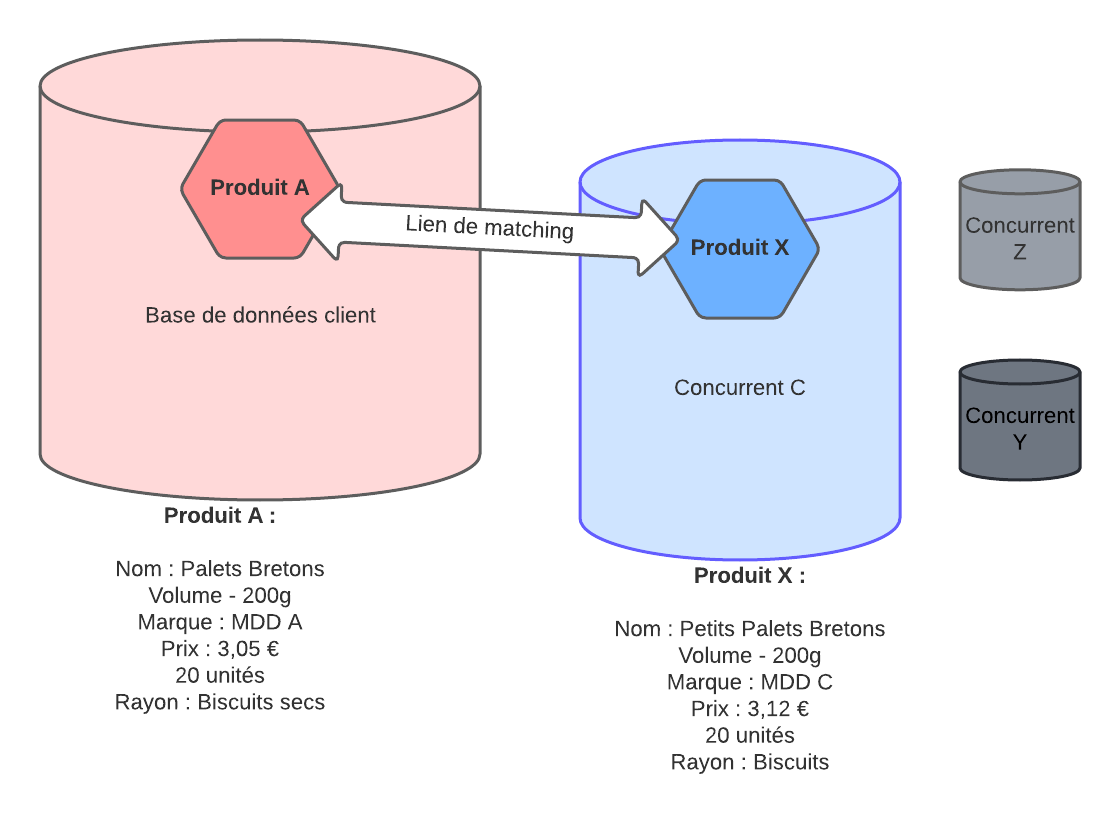
\includegraphics[width=20cm]{images/Matching1.png}}
  \caption{\label{Matching1} Exemple facile de lien de chaînage horizontal}
  \end{figure}

Mettons que l'on décide de lier un produit A de la MDD de son enseigne au produit X de son concurrent,
ayant pour marque la MDD de ce concurrent.\\
Le produit A et le produit X possèdent plusieurs caractéristiques comme un nom, des catégories, un volume,
un paquetage, une marque, un prix, et bien d'autres dans les faits.\\
Nous sommes ici dans le cas facile où le produit n'est pas exactement identique à celui de son concurrent,
mais le produit semble concorder aux attentes de l'alignement concurrentiel : il s'agit de produits de MDD
respectives aux deux enseignes dans les deux cas, acheter l'un ou l'autre semble revenir au même pour le
consommateur final.\\
Aussi, les noms sémantiquement désigne le même produit, l'ordre de grandeur du volume 
vendu en rayon est le même, les catégories concordent assez bien, etc.
Nous avons tout pour dire qu'il est cohérent d'aligner A sur X pour ce concurrent-ci. \\

Nous aurions eu un mauvais lien si le prix était le double chez le concurrent, ou que tout 
sauf le nom du produit concurrent concordaient.\\
Par exemple dans le cas du titre, lier 20 biscuits pour 3€ et 200g liés à 20 madeleines pour 3€ et 200g 
est une erreur que ne ferait jamais un humain,
mais qu'un algorithme qui ne regarde pas le titre pourrait faire.  

\subsection{Agilité}

Dans tout travail de production logicielle, il est nécessaire de choisir une manière de fonctionner
qui assure la qualité du logiciel, le délai de livraison, la possibilité de maintenance et autres. 
L'équipe Produit chez Mercio travaille en général avec les méthodes Agile et Kanban.
Pour travailler sur mon sujet, je suis introduit à ce mode de fonctionnement, et
je vais donc suivre le processus classique qu'utilise les développeurs de cette équipe.\\

Les principes de ce processus productif sont de :
\begin{enumerate}
  \item Sortir une version du Produit Minimum Viable (PMV) et fonctionnelle le plus vite possible contenant
  les fonctionnalités que l'on veut construire dans le logiciel.\\
  L'idée est de fournir vite un service incomplet, mais vendable,
  dans l'optique de le raffiner plus tard en fonction du besoin brut des utilisateurs.
  \item Laisser l'utilisateur faire des retours sur la première version livrée de ces nouveautés,
  afin de cibler avec précision le véritable besoin.
  \item Agrémenter le logiciel des changements proposés par leurs retours, 
  pour répondre à ces besoins en effet tunnel.\\
  Ainsi, on ne crée rien d'inutile dont l'utilisateur n'aurait pas besoin immédiatement.\\
  De plus, l'évolution du logiciel se déroule main dans la main avec le principal concerné, ce qui 
  crée chez lui un sentiment d'être écouté, une satisfaction plus régulière.
  
\end{enumerate}

Les étapes de production sont les suivantes :
\begin{enumerate}
  \item Créer un document appelé 'Epic' qui met en avant les changements / fonctionnalités à développer
  pour améliorer le service existant : 
  \begin{itemize}
    \item Pourquoi les changements proposés sont intéressants, 
    \item Quels utilisateurs sont concernés par les fonctionnalités,
    \item Combien de temps prends le développement des fonctionnalités. 
  \end{itemize} 
  À noter que ce type de document est accompagné d'User Stories (US), qui sont des descriptions des fonctionnalités
  à développer côté utilisateur. Par exemple : \\
  "En tant que client / utilisateur, je veux disposer de recommandations de liens pour me positionner 
  sur ma concurrence" est une US à laquelle on répondra par un développement ou ensemble
  de petits développements, chiffré en nombres jours, décomposé éventuellement en plusieurs
  US qui auront un développement atomique associé.
  \item Écrire les US correspondants à notre EPIC, qui précisent les conditions de leur propre complétude.
  \item Ouvrir les branches de développement des premières US. Une fois qu'une branche de développement est terminée,
  elle est soumise à la revue des pairs, puis doit être approuvée sous réserve de changements exigés par la personne
  de l'équipe qui passe le code en revue.\\
  Pendant que le code d'une branche est revu, une autre branche de développement associée à une autre US est ouverte.
  \item Continuer d'itérer sur les changements jusqu'à ce que les fonctionnalités soient complètes et qu'une
  nouvelle version les comprenant soit livrable à certains ou à tous les utilisateurs.
  \item Déployer une nouvelle version du produit et laisser les utilisateurs disposant des nouvelles fonctionnalités
  faire des suggestions ou se plaindre de bugs.
  \item Revenir sur les retours par l'intermédiaire de tickets : ces tickets ont des tags qui correspondent
  à une importance ou bien à une spécialité de développement.
  \item Les changements des tickets sont intégrés avec une vitesse relative à l'urgence du sujet qu'ils traitent.
  \item Recommencer.
\end{enumerate}

\subsection{Planification des travaux}
Après plusieurs phases de discussions autour du sujet, nous avons convenu d'une feuille de route
pour accomplir les objectifs sous-jacents. Le sujet s'insère dans une procédure Agile décrite plus haut.\\
L'ensemble des travaux se segmentent en étapes ordonnées comme suit :\\
\begin{enumerate}
  \item Prendre connaissances des données primaires à traiter, comprendre leur spécification.
  \item Associer les données à des connaissances métier.
  \item Formuler une intuition d'approche pour définir un périmètre de recherche de solutions sur le net.
  \item Référencer les approches similaires dans la littérature scientifique et les forums dédiés à la data science,
  dans l'idéal illustrées par du code, fourni avec un dataset proche du nôtre sur lequel 
  on peut reproduire les résultats.
  \item Rassembler les approches les plus prometteuses, les présenter et 
  se concerter pour choisir quelle solution algorithmique utiliser pour générer des liens de matching.
  \item Chiffrer les étapes en termes de durée pour les situer dans le temps.
  \item Pré-traiter les données afin d'avoir des informations exploitables pour la solution choisie.
  \item Construire des modèles et les tester. Éventuellement réviser le prétraitement au besoin.
  \item Évaluer les résultats et les communiquer.
  \item Implémenter une première version du module de matching avec les recommandations visibles, et
  avec possibilité de valider les liens proposés.
  \item Faire des tests approfondis en interne sur la nouvelle fonctionnalité.
  \item Raffiner l’algorithme qui génère les recommandations de liens.
  \item Déployer la fonctionnalité pour un ou plusieurs client(s) avec ses pipelines de traitement
  de ses données, établir un feedback.
  \item Donner plus d'actions possibles dans l'application par rapport aux recommandations de liens, à
  travers une v2 de la fonctionnalité.

\end{enumerate}

Pour la planification initiale des tâches à accomplir afin de mener à bien le sujet, je fais régulièrement des 
points avec Guillaume et éventuellement Yoann en même temps, pour discuter hebdomadairement des avancées, des
tâches à suivre, et d'autres aspects similaires concernant mon travail au sein de Mercio.
La feuille de route initiale, qui m'a aussi permis de chiffrer (de manière optimiste) la durée de ces tâches,
est éditée avec GANTT Project au fur et à mesure. \\

Parmis ces tâches, il y en a certaines qui avancent en parallèle au vu de leur nature,
comme la phase de recherche dans la littérature de solutions envisageables pour développer 
un algorithme, et la configuration de l'environnement Python aussi bien 
utilisé pour tester ces solutions que pour concevoir des modèles.\\
Ce dernier exemple figure sur le diagramme de GANTT ci-après :\\

\begin{figure}[h!]
  \centerline{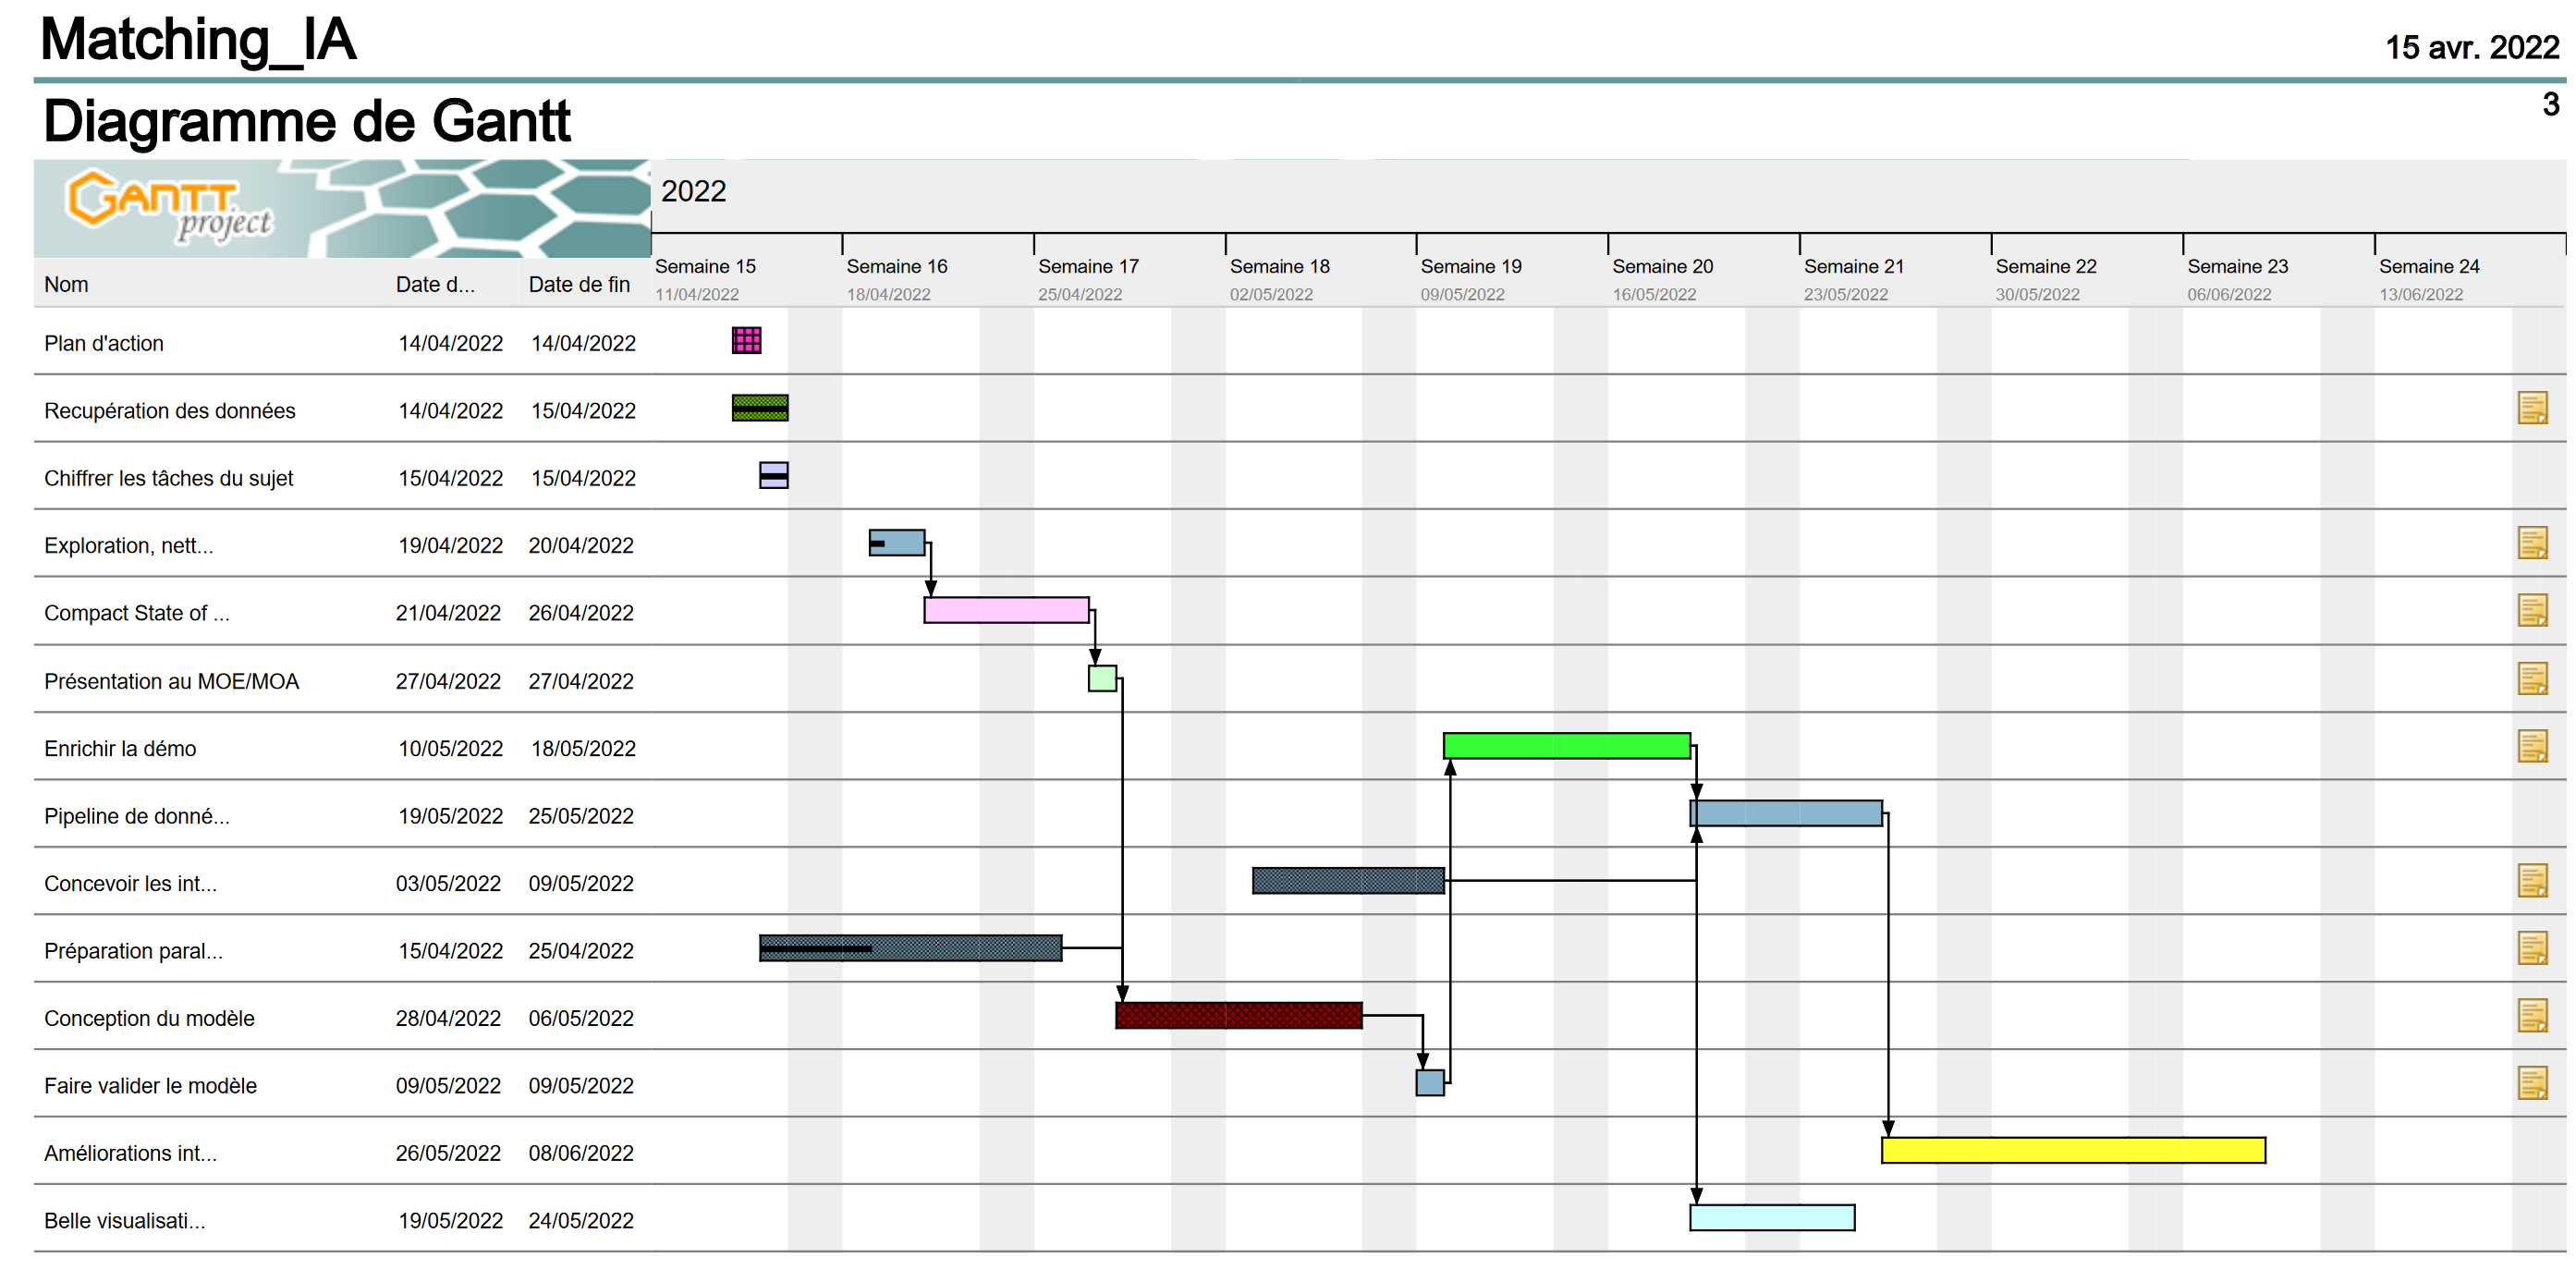
\includegraphics[width=20cm]{images/gantt_init.png}}
  \caption{\label{GANTT initial} GANTT Initial du sujet côté intelligence artificielle}
  \end{figure}

À noter que ce diagramme a évolué de multiples fois au fil des semaines de travail afin de refléter au mieux
l'écart final de mon estimation à faire certaines tâches et leurs durées finales, ainsi que les tâches dont 
l'exécution n'avait pas été anticipé de ma part.

\newpage

\subsection{Solutions possibles et leurs justifications}

\paragraph{Recherche scientifique sur le sujet}
Il y a plusieurs approches axée IA que j'ai examinées pour essayer de répondre à la problématique.\\
Toutes ces approches ont des avantages et des inconvénients pour arriver à ce but. On peut aussi éventuellement
combiner certaines de ces dernières.
Pour chaque approche, j'ai essayé des combinaisons de features \footnote[4]{Features : dans le sens des métriques
des données en entrée du modèle de machine learning} différentes pour certaines solutions.

\begin{enumerate}
  \item Approches non-supervisées :
  \begin{enumerate}
    \item Clustering + Calcul de distances au sein du cluster pour trouver le produit le plus proche
    pour chaque produit client.
    \item Réduction de dimension et clustering en même temps (UMAP) + calcul de distances comme décrit plus haut
  \end{enumerate}
  \item Approches supervisées :
  \begin{enumerate}
    \item Réseaux de Neurones Convolutionnel (RNC) avec Traitement Automatique du Langage (TAL)
    pour des mesures de similarité sur les titres des produits.
    \item RNC avec extraction de features du titre du produit grâce à d'autres techniques de TAL \cite{product_matching_ecommerce,xgboost}.
    \item Utiliser les liens déjà existants dans l'application pour entrainer un algorithme par renforcement.
  \end{enumerate}
\end{enumerate} 

Globalement, on tâche de prendre tous les produits client d'un côté et tous les produits concurrents de l'autre et
pour chaque produit client, calculer le produit concurrent le plus proche pour chaque concurrent différent.\\
On passe forcément par du calcul de distance dans des ensembles de produit 
(un par concurrent modulo les catégories que l'on identifie).\\
La distance entre deux produits est calculées en distance euclidienne sur les métriques trouvées pertinentes 
(trouvées notamment par l'intuition métier puis par l'étape de feature selection après).
On a toujours à gauche les produits clients et à droite les produits d'un concurrent.
Pour chaque concurrent, pour chaque produit client, on crée en sortie une suggestion de lien 
avec le produit le plus proche selon la méthode utilisée, sous-jacente au modèle choisit.

\paragraph{Discussion : approches clustering}
Le clustering présente l'avantage de ne pas nécessiter de données labellisées pour constituer des groupes
de données entre elles.\\
Cependant, l'hypothèse que l'on puisse établir des clusters cohérents
avec les métriques que l'on choisit pour nos instances de produits n'est pas toujours vérifiable.
Aussi, les produits ne sont pas tous susceptibles d'avoir toutes ces métriques renseignées,
à tel point que certains datasets de produits seraient en pratique inutilisable dans le cas où Certains
champs ne sont pas suffisamment renseignés.\\
Le clustering permet de réduire les espaces dans lequel on fait des calculs de distances entre produits.\\
Néanmoins, il est difficile de définir si un modèle non supervisé contribue in fine à produire de bons liens sans mesures
d'évaluation personnalisées à la tâche.

\paragraph{Discussion : approches TAL}
L'avantage, c'est que tous les produits présentent un titre dans tous les datasets mis à disposition. Cela
donne donc un aspect très adaptatif à beaucoup de jeux de données produit.
\cite{peeters_supervised_2022-1,product_matching_ecommerce}\\
Un autre avantage, c'est que l'on dispose de mesures déjà connues pour l'évaluation de l'algorithme tel que
la précision, le rappel et la mesure F1 (qui est une combinaison des deux premiers).\\
Un premier inconvénient, c'est que le fait de définir un vocabulaire sur des mots spécifiques à des intitulés de produits 
et non de vraies phrases semble assez houleux. En effet, les données de produits que j'ai à disposition pour faire les
tests sont remplies d'abréviations pour les clients, tandis qu'il n'y a pas les mêmes 
abréviations pour les données concurrentes.
Un deuxième inconvénient, c'est qu'une approche de la sorte peut être potentiellement plus lente à définir que 
les autres types d'approches décrites dans le précédent paragraphe, d'un point de vue conception.


\paragraph{Discussion : utiliser les liens déjà existants}
Cette approche est intéressante si on a déjà beaucoup de liens créés par l'utilisateur possesseur du dataset sur
lequel on travaille.\\
On a accès également au trio precision, recall, F1-measure.
Cependant, on ne peut donc pas suggérer de liens pour des utilisateurs qui n'auraient pas
encore créés de liens sur la plateforme, sauf les liens déjà faits ou simplistes avec le même EAN des deux
côtés.

\paragraph{Feature selection}
Une des étapes clés de la conception d'un algorithme de machine learning est la feature selection\footnote[5]{Étape
de choix des caractéristiques des instances à utiliser pour entrainer et prédire dans un algorithme de machine learning}, 
qui représente aussi l'occasion de faire du tri sur les données de mauvaise qualité.  

\paragraph{Open Food Fact}
Une première intuition formulée au tout début du stage était d'utiliser la base de données en accès libre
Open Food Fact pour se procurer davantage d'information sur les produits que la base de données possède en commun.
Cependant, on se cantonne aux produits alimentaires ce faisant.\\

On a accès aux catégories alimentaire des produits à différentes échelles, et on gagne des informations comme
le nutriscore et d'autres mesures concernant la composition des produits.\\
Toutes ces mesures aident à fournir plus d'entrées à l'algorithme, en plus de prodiguer des filtres supplémentaires.

\newpage
\section{Travail réalisé}
Le travail autour du sujet se divise en deux phases principales :
Concevoir une solution algorithmique de type machine learning pour générer de bons liens de matching,
puis intégrer les résultats de cette solution dans l'application web Mercio Pricing.
La deuxième étape qui inclus du développement logiciel est toujours en cours.\\
Cette dernière est elle-même scindée en trois parties :
\begin{itemize}
  \item Charger les liens recommandés côté serveur depuis une base de données,
  \item Créer les opérations côté serveur pour que l'Interface Utilisateur (UI)
  puisse interagir avec les liens recommandés chargés,
  \item Apporter des modifications côté UI pour que les utilisateurs de Mercio Pricing
  puissent interagir avec les recommandations de liens issues de l'algorithme de machine learning.
\end{itemize}

J'ai donc travaillé non seulement sur l'algorithme et sur son paramétrage,
mais également sur l'implémentation logicielle de ce dernier.

\paragraph{Travail data science}
J'ai testé principalement des approches non supervisées dans l'optique d'obtenir rapidement des résultats 
globalement satisfaisants, quitte à revenir dessus une fois qu'une première phase
de l'implémentation logicielle sera mise en place avec succès.

Au moment où je rédige la fin du rapport j'en suis au moment où je termine l'interface
utilisateur du module de chaînage horizontal pour la branche en production.


\subsection{Analyse de la tâche}

\paragraph{Retour critique sur mes travaux}

Pour tester la précision d'algorithme d'intelligence artificielle, on utilise très souvent des mesures pour
nous indiquer si les prédictions réalisées sont correctes dans l'ensemble. En choisissant le clustering
comme première approche, je me suis rendu compte que l'on ne peut compter que sur la pureté des clusters
et la densité de ceux-ci.
Comme le résultat final de la pertinence des liens ne dépend pas de ces indicateurs, on peut se poser la question
suivante : a-t-on vraiment besoin de grouper les produits sachant que les groupes ne servent qu'à réduire
le temps de calcul d'un simple calcul de distance ?\\

De simples filtres sur les catégories extraites d'Open Food Fact pour les produits qui disposent de l'information,
auraient été plus efficaces pour regrouper les produits de manière cohérente. C'est ce que m'avait conseillé mes
maîtres de stage dans les premiers instants de l'élaboration de l'algorithme qui génère les liens.\\

Seulement j'ai un peu voulu faire de l'IA juste pour en faire, sans que l'apport soit suffisant d'un point 
de vue calculatoire.\\
Cependant, grâce à cette expérience, j'ai pu imaginer des solutions plus pertinentes à mettre en place,
qui ne sont pas très éloignées des approches de traduction automatique, mais appliqué à des titres de produits d'un catalogue
à un autre.\\
En effet, on peut très bien filtrer les produits selon leur appartenance à une MDD dans les deux camps (client et concurrence),
filtrer selon la cathégorie ou le rayon dans les deux camps, puis pour chaque catégorie :\\

\begin{itemize}
  \item tokkeniser les titres des produits ;
  \item constituer un vocabulaire avec uni-grammes et bi-grammes ;
  \item choisir des mesures de similarité (string-based et sémantiques) ;
  \item mesurer deux à deux tous les produits clients aux produits concurrents ;
  \item créer des liens avec les produits deux à deux les plus proches.
\end{itemize}
C'est une idée de démarche à mettre en œuvre, certes incomplète, mais le matching de produits
reste une tâche en $O(n^2)$. \\

Quant à la partie développement logiciel, sur laquelle je travaille encore actuellement, elle a été bénéfique, car 
j'ai appris sur les habitudes des utilisateurs et leurs attentes. C'est en travaillant dessus que j'ai réalisé
que simplifier au maximum la démarche, quitte à se séparer de l'IA sur certains calculs, est toujours une bonne
option à prendre pour aller vite au but.


\subsection{Résultats expérimentaux, tests}
\paragraph{Partie algorithme de machine learning}
Les clustering KMEANS, DBSCAN, UMAP ont été essayés dans cet ordre pour
tenter d'obtenir des résultats avec des clusters cohérents pour nos calculs
de distance entre produits.\\
À noter que UMAP se distingue des deux premiers, car il fait aussi de la réduction
de dimensions + standardisation des features en même temps.
Par ailleurs, c'est un algorithme très utile pour mettre à plat les données afin de mieux les visualiser.\\

Pour évaluer les résultats d'algorithmes de clustering, dans le cas général,
on possède des mesures d'homogénéité intra-cluster et inter-cluster intégrées à la bibliothèque
d'apprentissage non supervisé de SciKit-Learn.\\

J'utilise diverses features pour faire fonctionner ces algorithmes.\\
On peut visualiser leur taux de corrélation via une heatmap :
% include heatmap
Il y a celles obtenues d'Open Food Fact et celles qui proviennent
des données de base (client + concurrents).\\
Provenant d'Open Food Fact, j'ai choisi de récupérer les métriques qui suivent, en
fonction de taux de disponibilité sur l'ensemble du dataset :
\begin{itemize}
  \item Taux de gras, de gras saturé, de protéines, sucres, fibres, sel, énergie, tous pour 100g ;
  \item Le nutriscore brut (en chiffres, non converti en lettre).
\end{itemize}

Provenant des bases de données internes, j'ai choisi de prendre en compte
ces métriques de produits :
\begin{itemize}
  \item Leur typologie : appartenance à une MDD ou MN ;
  \item Leur prix de vente moyen ;
  \item leur volume.
\end{itemize}

Au niveau des données client, j'aurais pu prendre aussi d'autres métriques
intéressantes comme le taux de marge,
en agrégeant des données provenant d'autre site de stockage.
Cependant, je n'aurais sans doute pas eu l'équivalent dans les données de la concurrence.\\

Les modèles sont entrainés avec les données concurrentielles et
les prédictions sont faites avec les données client.\\
Ensuite, nous calculons pour chaque produit client le produit concurrent 
le plus proche au sein du même cluster, pour chaque concurrent.

Le point faible des algorithmes de clustering est la présence de bruit dans les
données. Pour lutter contre ce phénomène, j'utilise un modèle de prétraitement
appelé Isolation Forest qui supprime les produits qui ont des métriques anormalement
élevées (on parle de "outliers").\\

\paragraph{K-Means et DBSCAN}
Afin de faciliter le calcul pour le clustering,
j'ai eu recours à des méthodes de réduction de dimensions.
Pour réduire les dimensions dans KMEANS et DBSCAN, j'ai utilisé de l'Analyse en Composantes
Principales (PCA) et j'ai aussi utilisé UMAP a posteriori pour l'affichage 2D des résultats.\\

À noter que toutes les features sont standardisées au préalable, certaines non numériques sont
encodées avant la standardisation \cite{cathegorical_data}, comme la typologie.

% k means include
\begin{figure}[h!]
  \centerline{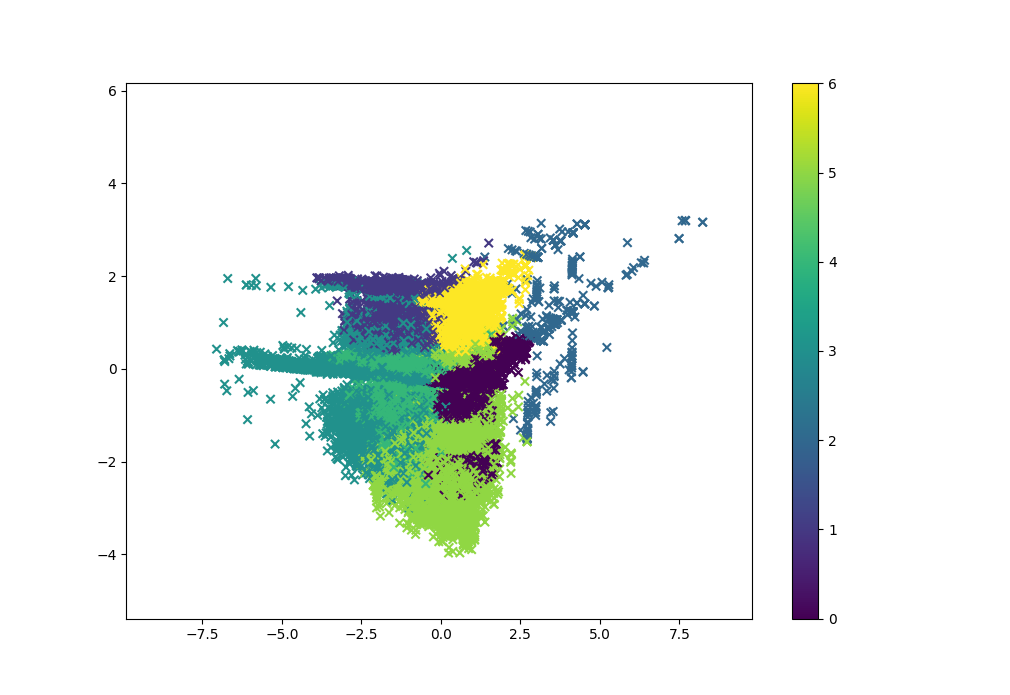
\includegraphics[width=20cm]{images/Kmeans_seven_clusters_pca_new_features.png}}
  \caption{\label{K Means PCA} K-Means pour prédire le cluster des produits clients après PCA}
  \end{figure}

C'est à cette étape que l'on peut, avant de passer à l'étape du calcul de distance intra-cluster 
pour les produits passés en prédiction, vérifier que nos algorithmes ont des clusters bien homogènes.
Je décide d'abord de tester un dernier algorithme avant de me lancer dans une potentielle évaluation
de la tâche, car je ne suis pas sûr du lien de causalité suivant :\\
\textit{Un algorithme de clustering qui a de bons indices d'homogénéité intra-cluster et inter-cluster
sera apte à nous donner de bons liens de matching lors de l'étape de calcul de distances entre 
produits concurrent au sein du même cluster.}\\
De plus, les features étant toujours nombreuses après la PCA, je me dis qu'UMAP peut aider pour l'étape
finale de calcul de distances grâce à sa réduction de dimensions efficace.

\newpage

\paragraph{UMAP}
Comme précisé plus haut, UMAP transforme les données par paquet tout en réduisant leurs
dimensions ; le nombre de dimensions et la taille de ces paquets dépendent du paramétrage.

% include umap
\begin{figure}[h!]
  \centerline{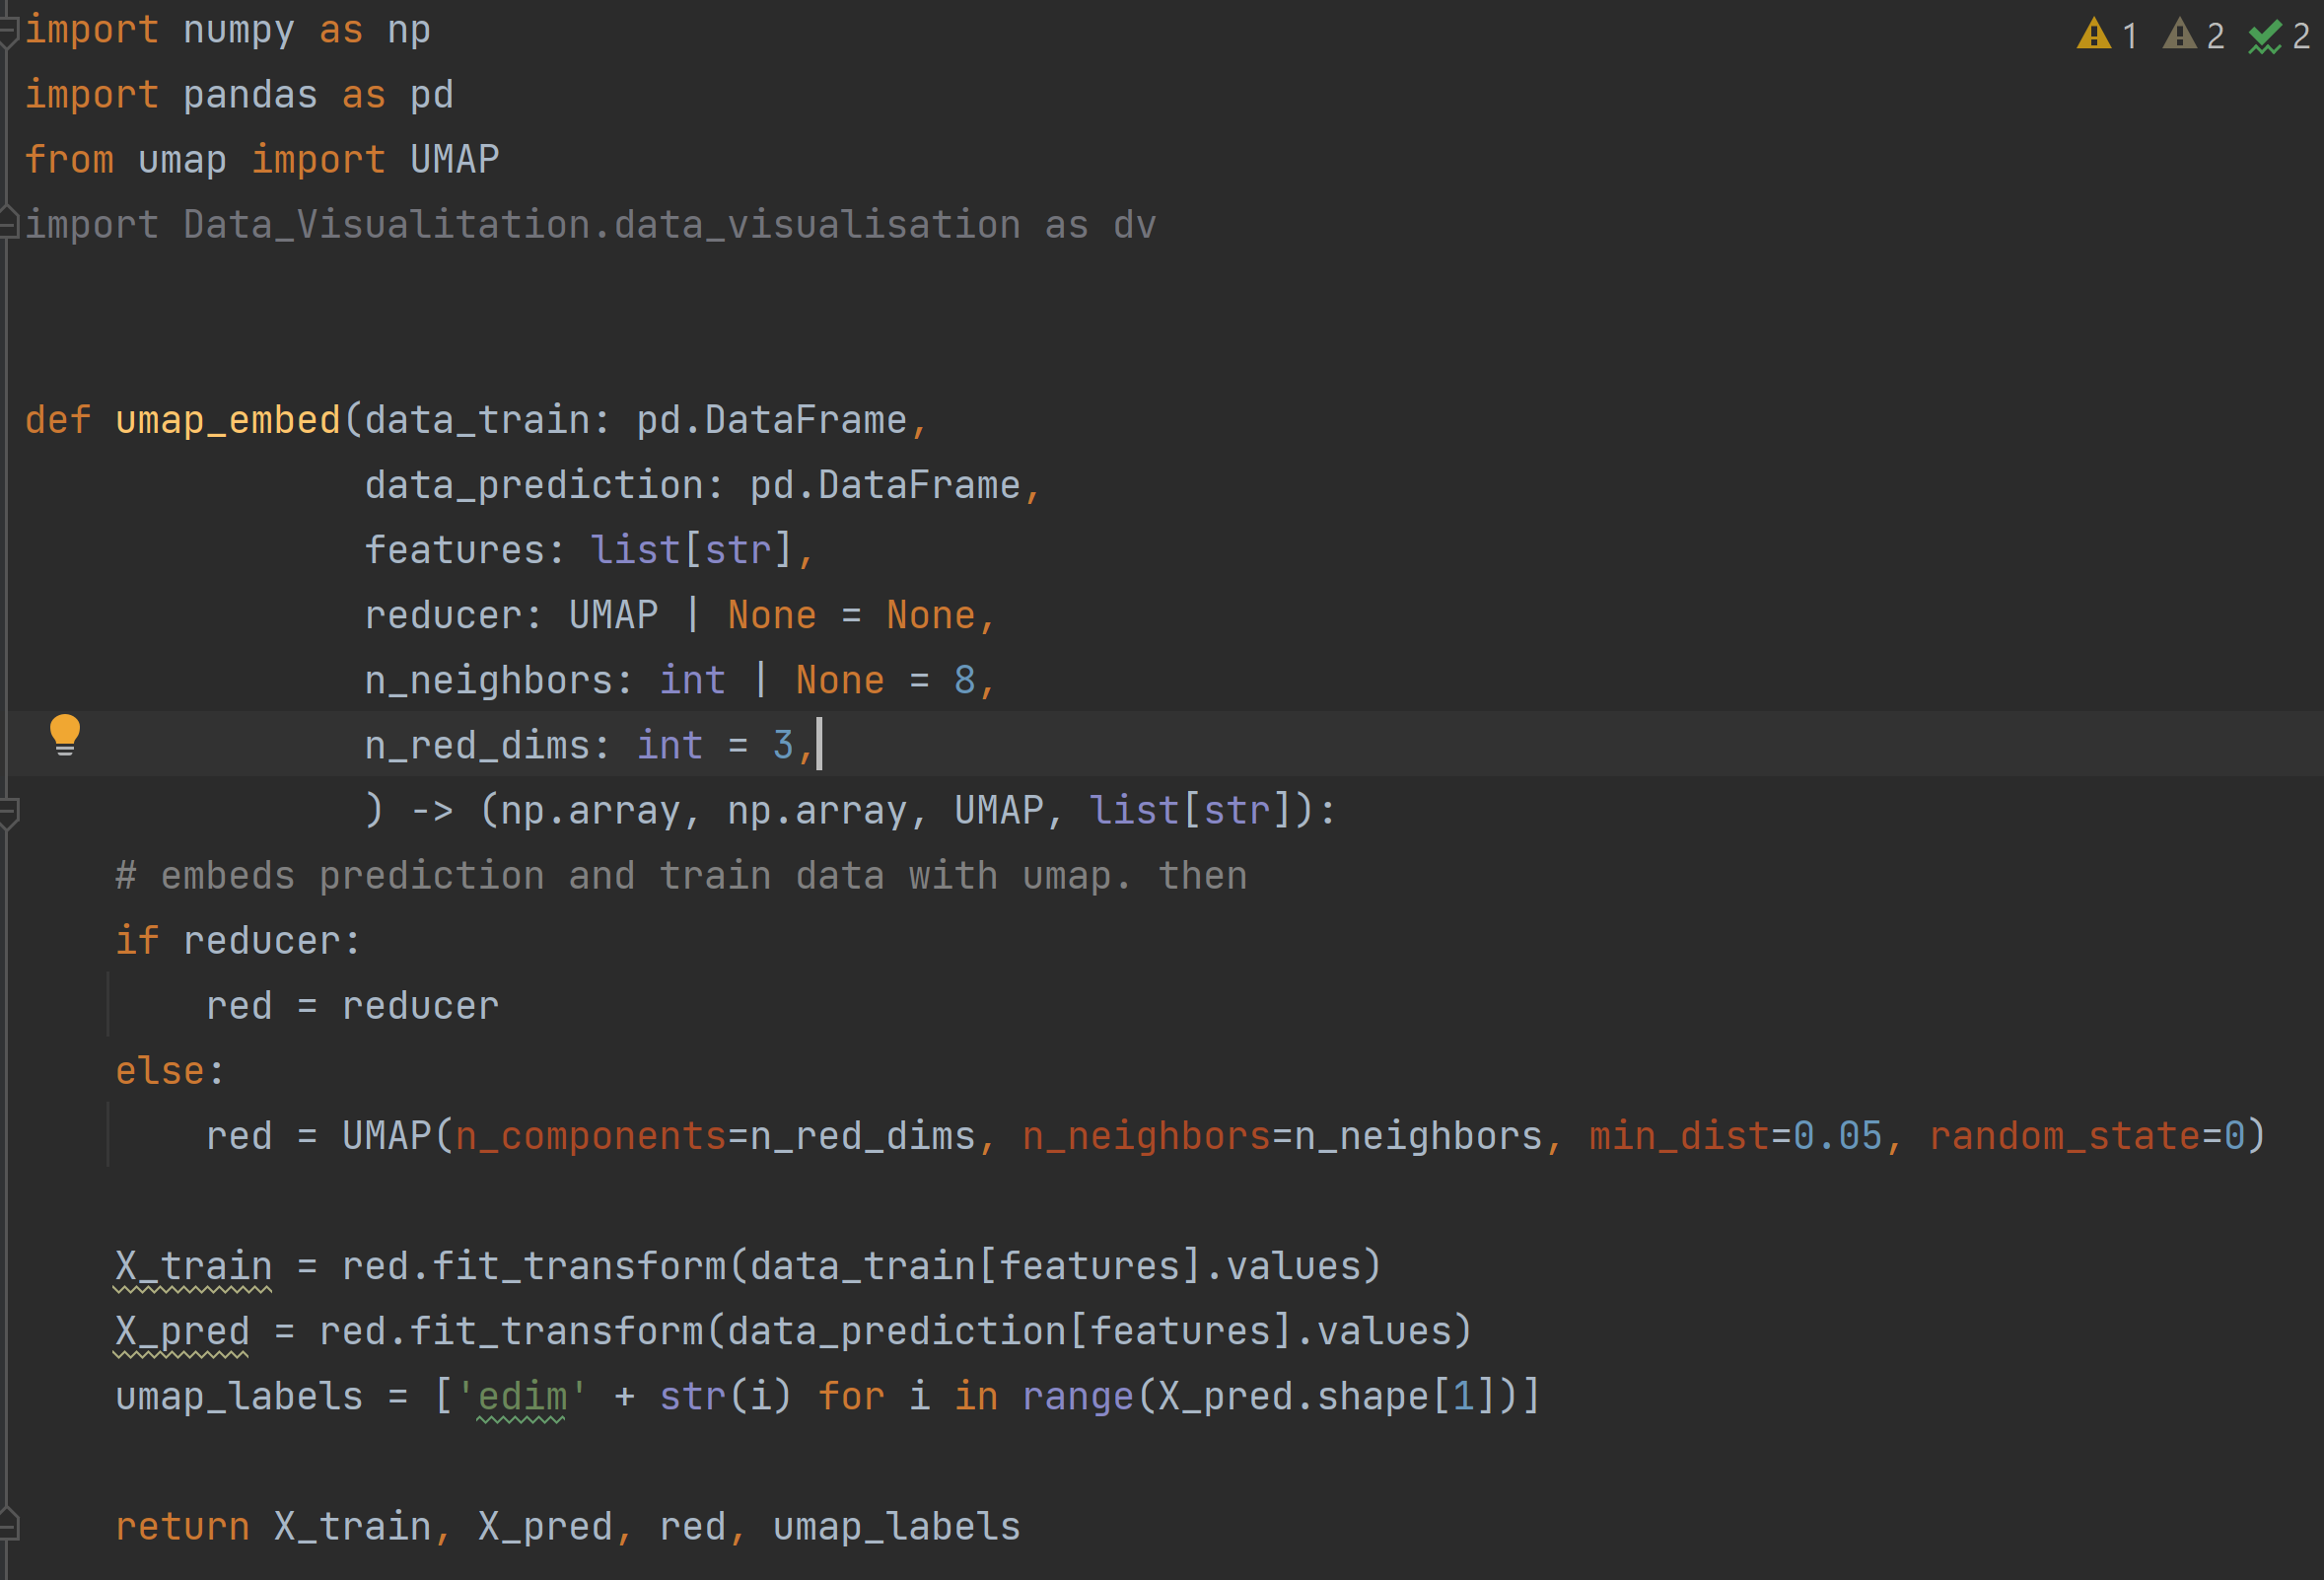
\includegraphics[width=20cm]{images/code_umap.png}}
  \caption{\label{Code umap} Code pour la production de dimensions réduites + groupage de données en simultané avec UMAP}
  \end{figure}

C'est sur ce dernier algorithme que j'ai décidé de tester de calculer les distances
entre produits au sein du même cluster, après prédiction.\\

Les résultats n'étant pas très concluants, j'ai observé beaucoup de résultats à
la main pour voir les liens que nous ressort l'algorithme après le calcul de distances.\\
C'est à ce moment-là que j'observe un fort biais sur les données, notamment la métrique de Volume
qui a tendance à faire correspondre des produits qui n'ont rien à voir entre eux.\\
J'ai appris plus tard que le Volume d'un produit n'est en effet pas pertinent d'un point de vue métier comme 
critère de matching : le packaging d'un produit d'un magasin à un autre varie et influence leur volume total
en base de donnée, sans que le contenu du produit ne change.\\
Le nutriscore brut est aussi source de confusion, car un nutriscore de 0 est aussi équivalent d'un nutriscore
non référencé ou 'non applicable' dans la base de données Open Food Fact.\\

Je remarque qu'aussi, je sample mal les données d'entrainement et les données de prédictions.
Comme on travaille avec des dizaines de milliers de produits, il faut être précautionneux lorsque l'on
prend seulement un pourcentage des produits chez le client à faire correspondre à la concurrence.\\
Plus précisément, il vaut mieux se restreindre à une seule catégorie de produit pour vérifier nos
performances sur un échantillon de données, que de faire un échantillon à base de lignes aléatoires
du fichier source. Sinon, on n'est pas garanti que l'on puisse relier quoi que ce soit de cohérent.\\
Encore faut-il avoir une information commune de la catégorie des produits, ce qui n'est pas toujours
le cas.\\

C'est à ce moment-là que je commence à réaliser que les approches à base de TAL,
que ce soit supervisées ou non, ont un réel intérêt,
car les métriques ne dépendent pas autant du choix des features quand on se focalise seulement
sur les noms des produits, en plus de ne pas nécessiter de jointure au préalable pour fonctionner.
Et ce, même si les noms des produits sont très mal écrit pour le client, grâce à des techniques 
de prétraitement \cite{xgboost} on peut largement s'en sortir.\\

\paragraph{Déductions de l'expérience}
Je ne regarde pas les métriques sur la formation des clusters pour les différentes expériences, car
j'identifie que l'approche ne se base pas sur les bonnes données à cause d'exemples flagrants comme 
décrits ci-dessus, ou n'est pas aussi pertinente qu'imaginé, ou n'est pas assez bien 
paramétrée sur le nombre de clusters, leur taille maximale, etc.\\

Aussi, il y a une nécessité de définir des mesures de précision pour la prédiction de liens après
calcul de distance. Tant que ces mesures ne sont pas complétement définies, on ne peut pas
réellement juger de la qualité de notre algorithme de clustering.\\
L'objectif final reste de générer des liens entre produits en calculant pour chaque produit client, 
le produit concurrent le plus proche classé dans le même cluster lors du training.\\
Pour cette mesure de précision, je propose d'inclure la distance avec laquelle un lien est trouvé,
comparé à la distance maximale qu'a produit le plus éloigné du cluster.\\

Cependant, bien que qu'une mesure de précision soit nécessaire pour évaluer la pertinence d'un lien généré,
je ne suis pas sûr que ce genre d'évaluation (ou du moins celle que je propose)
soit pertinente dans une approche non supervisée.\\

Quand bien même je décide de présenter mes résultats et de passer à la partie développement logiciel du 
sujet, quitte à revenir sur une approche différente plus tard.\\
En effet, je suis resté longtemps sur la fin à changer d'algorithme plusieurs fois alors
que j'aurais pu calculer les distances intra-cluster dès les premiers tests sur K-Means.
Donc, je passe à la suite.

\paragraph{Partie développement logiciel}
Pour l'implémentation serveur et au niveau UI de la partie développement de mon sujet,
le déploiement ne se fait que sur la partie locale de l'application destinée au développeur.\\
Cependant, si un client a sa version de l'application avec la bonne option de configuration,
il aura dans son module de matching la vue correspondante aux recommandations que je suis
en train de mettre en place.\\

Je ne détaillerai pas les travaux courants qui concernent l'UI que je modifie actuellement pour que l'utilisateur
accède aux recommandations de liens.\\

%conf screen UI annexe confidentielle 4.a
Voici l'avancée actuelle du développement où seront intégrée les recommandations de liens trouvées avec
l'algorithme de génération automatique de liens de matching :\ref{confidentiel} \\

\newpage
\paragraph*{Développement en Java SpringBoot}
Côté serveur de l'application, je me suis fortement inspiré de ce qui était déjà fait
au niveau des liens pour charger en bases de données mes liens recommandées.\\

Premièrement j'ai conçu le modèle de données en fonction de ce qui était déjà présent,
puis j'ai commencé à créer les objets de mes liens recommandés.
Grace aux modules JPA, ils seront stockés dans une base de données relationnelle,
et on définit à l'intérieur des classes l'arité des relations avec les autres tables.\\

%include rela
\begin{figure}[h!]
  \centerline{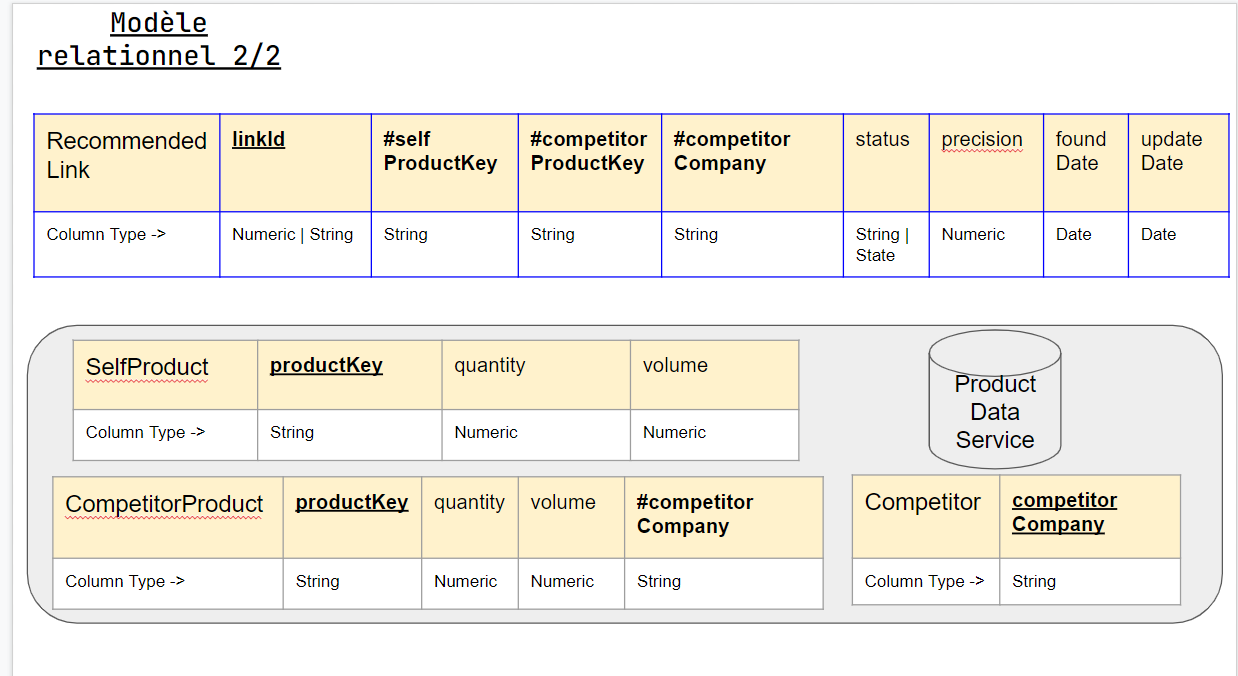
\includegraphics[width=20cm]{images/relationnel.PNG}}
  \caption{\label{relationnel} Schéma relationnel pour l'ajout des liens recommandés dans le serveur}
  \end{figure}

Ensuite, j'ai conçu les opérations consistant à récupérer les liens recommandés à partir de clé produits,
ainsi que celles qui permettent de créer de vrais liens par validation de ces recommandations.
Le tout, par l'intermédiaire de requêtes lancées au serveur. Ces requêtes sont des appels REST, qui sont
d'ordinaire lancée par l'application web au serveur, puis le serveur envoie sa réponse sous forme d'objets.\\
Lors de la conception de ces opérations, il est important de s'assurer que notre code est optimisé pour
faire le moins de requêtes possible à la base de données.\\
Sinon, on risque de gros problème de latence sur la réponse de notre serveur.\\

Le fonctionnement de tout ceci est assuré par des tests unitaires à plusieurs échelles,
qui tournent lorsque l'application est construite.
Alternativement, on peut simuler les requêtes REST via d'autres outils comme Postman 
(outil sympathique en développement Full-Stack),
pour vérifier si notre serveur fonctionne comme on l'entend.\\

\newpage
\section{Bilan de production}
\subsection{Objectifs atteints}

Un module Python comprenant toutes mes tentatives d'approches machine learning non supervisées est
disponible dans le GitHub de l'entreprise.\\
Un notebook Python y retrace la démarche et offre un exemple des étapes de pre-processing, d'entrainement
des différents modèles testés et quelques représentations graphiques des résultats.\\

Du côté développement logiciel, des parties de mon travail sont déjà intégrées à l'application et la partie
recommandation du module de chaînage horizontal va sans doute rentrer dans une nouvelle release avant
la fin du stage, le 30 septembre.\\

\paragraph{Avancée relative}
Ma principale phase d'apprentissage avec les technologies à manipuler est terminée,
ce qui veut dire que j'avance beaucoup plus vite sur tout ce que je fais à partir de maintenant.
Au début, je prenais beaucoup de temps à tout faire, car je débutais sur une démarche complète avec
beaucoup d'autonomie, mais j'ai mis des processus en place afin de gagner en confiance en moi, donc 
aussi en productivité.\\
Ainsi, je peux réitérer sur tous les points précédemment abordés avec plus d'expertise.\\
Ce qui me permettra, j'espère, d'avoir l'occasion de revenir sur la partie machine learning avec 
des approches plus efficaces, et d'avoir les premiers retours utilisateurs sur les
fonctionnalités déployées.


\subsection{Apport du travail réalisé}
Même si mon travail sur l'aspect intelligence artificielle est largement incomplet, le code de mes travaux peut
toujours être réutilisé pour prolonger les recherches sur ce sujet ou pour l'adapter à de futurs travaux.\\
S'il n'est pas amélioré sur les prochaines semaines de stage, il peut toujours servir en
récupérer les modèles de machine learning, la structure du programme de génération de lien
ou autres éléments de pré-processing des données.\\

D'un autre côté, les apports sur le serveur et l'UI de l'application sont réels et permettront aux utilisateurs
de Mercio Pricing de gagner du temps lors de leur parcours sur le module de chaînage horizontal, donc de 
répondre plus facilement à leur besoin d'alignement à la concurrence. 

\subsection{Perspectives d'évolution des travaux}
\paragraph{Travaux nécessaires restants}
Au moment de l'écriture du rapport, il reste 8 semaines de stage dont les dernières seront consacrées à :
\begin{enumerate}
  \item Terminer les modifications sur l'UI du module de chaînage horizontal,
  \item Implémenter la validation de lien recommandés dans l'application,
  \item Revenir sur l'algorithme de génération de liens,
  \item Définir les processus qui permettent aux clients d'avoir automatiquement ces liens recommandés
  pour tous types de produits.
\end{enumerate}

\paragraph{Discussion sur les tâches restantes côté produit}
Selon le fonctionnement du processus Agile, on peut aussi imaginer que lorsque cette version
du nouveau module sera mise en production, toutes les fonctionnalités relatives aux recommandations
de liens seront sujettes à être améliorées après retour des utilisateurs. \\
Je pense notamment au fait de pouvoir rejeter des liens si jamais les deux produits ne sont pas
pertinents à relier, ou bien de pouvoir choisir un autre produit,
afin de ne pas les avoir proposés à nouveau dans un contexte de bon parcours utilisateur.

\begin{figure}[h!]
  \centerline{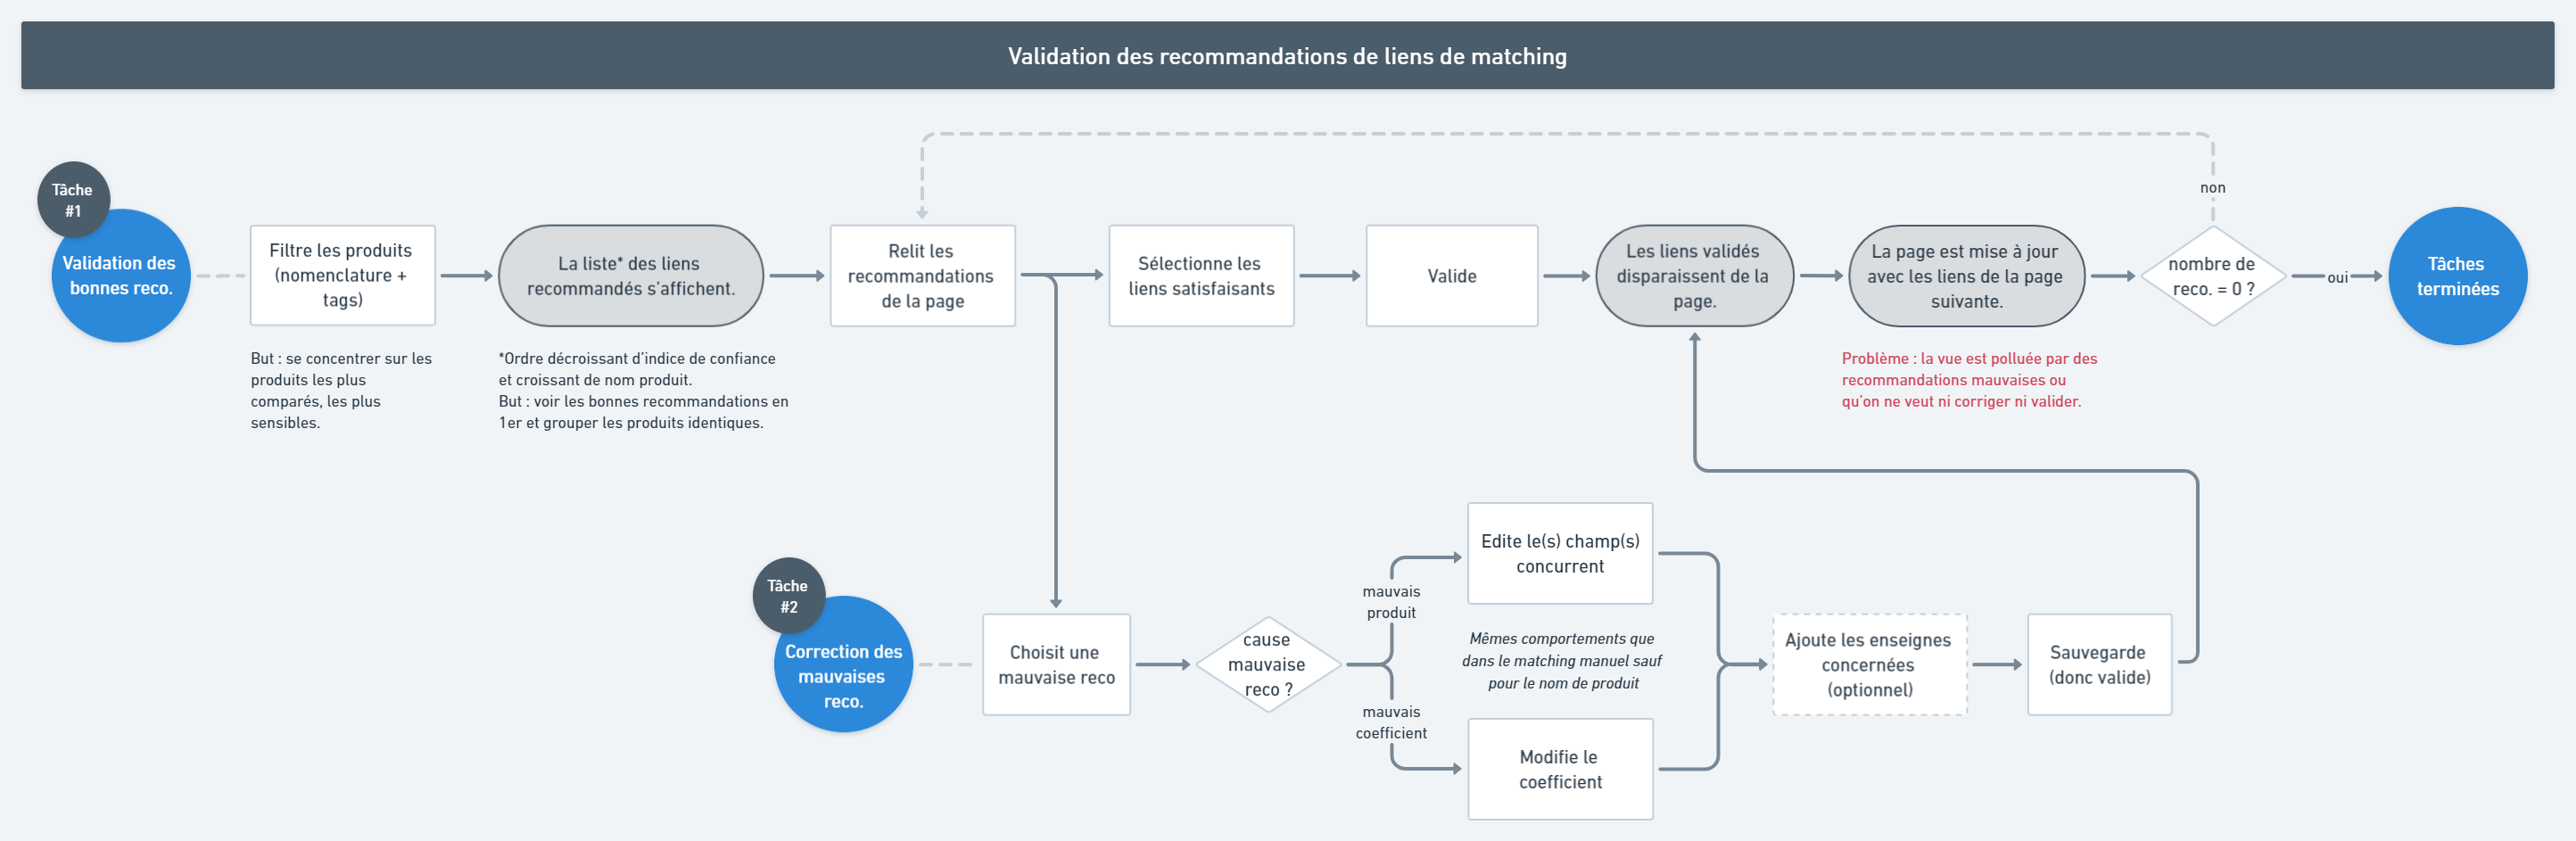
\includegraphics[width=20cm]{images/parcours_ux.png}}
  \caption{\label{Parcours UX} Parcours utilisateur pour les liens recommandés, par Magalie, UX designer}
  \end{figure}

\subsection{Bilan général de la démarche}

Avec le retour sur les travaux lié à la rédaction sur le rapport,
plusieurs points sur lesquels on peut revenir apparaissent.\\
\begin{itemize}
  \item La méthodologie scientifique appliquée pour répondre à la problématique,
  \item L'effet de la démarche sur l'avancée des travaux,
  \item L'inclusion dans le processus de production de l'entreprise.
\end{itemize}

\paragraph{Point de vue méthodologie scientifique}
La méthodologie qui a été suivie peut être critiquée à plusieurs points de son déroulement.\\
Le premier point à aborder est celui de la direction que j'ai prise après le choix
d'un algorithme non supervisé.
Il a en effet des articles scientifiques qui mentionne le non supervisé pour de l'alignement
produit, \cite[cf ces articles.]{akritidis_clustering-based_2019,ristoski_machine_2018,kaul_automatic_nodate,akritidis_effective_2018}
\\
Cependant, elles utilisent des approches axées Natural Langage Processing (NLP), ce que je pensais 
pouvoir être non nécessaire vu qu'avec les jointures sur Open Food Fact, on se retrouve
avec des métriques assimilables par un algorithme de machine learning.\\

Sur le papier, aller chercher des exemples sur le net d'approches similaires pour ensuite 
tenter quelque chose qui en diverge est un peu trop audacieux.\\
Par manque de compréhension sur les spécificités des données dans le retail, j'ai
fait des choix qui me paraissent maintenant plus que questionnables pour une
première approche.\\
Le fait d'avoir poussé la piste du clustering pour réduire les temps de calcul puis
de calculer les distances entre produit catalogue à catalogue,
n'est en fait pas plus pertinent qu'un simple travail sur les données pour appliquer des 
filtres avant ce calcul de distance. Seule la réduction de dimension a, elle, un certain
intérêt pour faciliter le calcul de distance entre produits de métriques communes,
client et concurrents.\\

Avoir choisi la simplicité m'aurait en plus permis de :
\begin{itemize}
  \item Respecter l'intuition de mes maîtres de stage dans l'utilisation d'une base
  de données tierce pour obtenir des catégories qui surclassent largement les clusters ;
  \item Éviter le nettoyage de données et la feature selection sur des caractéristiques
  issues d'une base de données qui n'est utile que pour l'alimentaire est qui n'avait
  jamais autant de produits en commun avec le client que ce qu'on espérait ;
  \item Me retrouver sans réelle documentation sur l'approche spécifique que j'ai choisi,
  alors que les approches existantes sont naturellement plus documentées.
\end{itemize}

Bien qu'ayant permis de pousser la réflexion dans des terrains inexplorés,
la démarche que j'ai suivie pour les travaux me laisse sur ma faim d'un point de vue 
scientifique à cause du manque de résultats solides, mais surtout,
car mon pari de penser en obtenir sans appliquer les techniques documentées est 
dû à mon manque d'expérience dans une démarche complète de recherche et développement.

\paragraph{Mesurer l'impact sur la productivité}
Open Food Fact est un dataset long à pré-traiter, car il est alimenté par des utilisateurs 
différents et qui remplissent parfois mal certains champs.
Aussi, c'est un programme de reconnaissance de texte sur les photos qui rempli les champs
pour la composition des produits, ce qui donne parfois des ratés sur les infos produit.\\

L'idée, c'est que plus on veut utiliser un dataset de ce type, plus il faut faire de prétraitement.\\
Tout le travail lié à ce prétraitement pour qu'un algorithme de machine learning non supervisé
fonctionne dessus, ne paie pas forcément si l'approche sur laquelle on part n'a pas fait ses preuves.\\
Je dirais que ces efforts sont, en pratique, largement devancés par une compréhension 
plus en profondeur des données traitées 
et de leur utilisation quotidienne qui en est faite par les professionnels concernés.\\

Avoir pu réitérer plus tôt sur une solution alternative plus robuste, quitte à
n'avoir pas utilisé de techniques d'IA du tout en premier lieu, était en fait
beaucoup plus cohérent que ce que j'aurais imaginé.\\

\paragraph{Une démarche axée production}

L'équipe dans laquelle je travaille vise un temps minimal de recherche
pour passer le plus vite possible à des résultats concrets.\\
C'est tout à fait normal pour une entreprise pour laquelle le temps qui n'est
pas passé à produire de la valeur de vouloir implémenter rapidement des solutions
quitte à revenir dessus plus tard. C'est la méthode Agile qui veut ça,
en opposition au modèle Waterfall ou cascade en français.\\
Là où je travaillais en cascade sur l'algorithme de génération de liens,
je pense qu'adopter très tôt et complètement le fonctionnement Agile m'aurait 
permis de palier mon manque d'expertise sur le domaine métier.\\
Ainsi, j'aurais pu arriver plus vite à un algorithme qui répond au besoin
plus tôt, j'aurais travaillé de manière plus pragmatique tout en suivant
mieux les directives.

\newpage
\section{Bilan sur le plan personnel}
Tous les enseignements qu'il m'a été donnés de recevoir sont extrêmement précieux en tant que
professionnel de la data, mais aussi en tant que travailleur tout court.\\
Le fait est que j'ai maintenant de vraies clés pour aborder les problématiques sur 
lesquelles je me suis heurté sans le savoir au début du stage.\\
Ces compétences réellement acquises ou solidifiées lors de ces quelques mois de stages
me suivront tout au long de ma carrière.

\subsection{Compétences mises en avant}
Il y a deux types d'atouts professionnels que j'ai développés lors de ce stage : des 
compétences techniques brutes, comme la maîtrise de techniques de
programmation par exemple, ou bien des compétences plus générales comme la 
communication en entreprise parmi bien d'autres.

\paragraph{Compétences améliorées}
Parmi les compétences non techniques abordées lors de mes études et que j'ai eu l'occasion
d'améliorer, on peut citer celles-ci :
\begin{itemize}
  \item \textbf{La prise de parole et la communication} sont des points que j'ai tâchés
  de mettre en exergue lors de multiples occasions. On peut citer par exemple
  les réunions hebdomadaires du vendredi où je présente les résultats de la semaine,
  accompagnées de temps en temps de slides. C'est un bon exercice en plus de 
  donner de la clarté à mon travail.
  \item \textbf{L'organisation au travail}, en particulier dans ce qui est
  de mettre des priorités ou de séquencer des tâches. Découper son travail en
  plusieurs petits objectifs atomiques sert à gagner en productivité, mais aussi
  à être sûr que ce que l'on fait s'intègre dans une démarche globale.\\
  J'utilisais régulièrement Trello au niveau personnel ou les espaces dédiés
  sur GitHub, ou bien sur le drive de l'équipe produit 
  pour communiquer sur les tenants et aboutissants de mes travaux en cours.
  \item \textbf{Du recul sur mes productions} est quelque chose que je n'avais que
  rarement lors de mon parcours universitaire, car il est rare d'avoir
  un retour détaillé sur le code que l'on produit à des fins d'évaluation.\\
  Quand du code doit être exécuté régulièrement par des utilisateurs exigeants,
  on y applique un cahier des charges strict. Ce qui implique des retours sur nos
  productions afin de garantir la qualité, la pérennité et l'adaptabilité du code que l'on
  écrit. Se détacher de l'effort pour se concentrer sur ces dernières, 
  réagir positivement à ces retours en toute circonstance, les voir comme autant de chances
  de s'améliorer, est quelque chose qui s'acquiert et se perfectionne.
  \item \textbf{S'intégrer dans une équipe} est obligatoire en entreprise, car on travaille
  tous ensemble pendant un espace de temps long et soutenu, sur plusieurs tâches distinctes,
  ce qui n'est pas toujours le cas dans les études, ou du moins pas à cette ampleur. 
\end{itemize}

Il y a aussi des compétences techniques que j'ai pu grandement perfectionner, toutes
très valorisées dans le monde du travail :
%mettre en avant utlité des competences + niveau de répendu dans 
\begin{itemize}
  \item \textbf{Faire du traitement de données en Python} en particulier avec les 
  bibliothèques pandas et numpy m'a été particulièrement utile pour rendre les données
  aptes à être utilisées dans le modèle de machine learning.\\
  Il y a eu plusieurs unités d'enseignements du master données et connaissances qui permettent
  de s'exercer sur ces aspects-là, mais finalement, chaque type de données doit recevoir un
  traitement spécifique afin de pouvoir faire quelque chose avec.\\
  En IA, Rendre digeste des informations de produits physiques pour un algorithme est une tâche
  qui diffère beaucoup selon les habitudes métier et le type d'algorithme qu'on pense pouvoir
  utiliser.
  \item \textbf{Concevoir un modèle de machine learning} avec Scikit-Learn, une bibliothèque
  Python pour faire de l'intelligence artificielle et bien plus encore autour de ce domaine.\\
  J'ai pu utiliser les principes calculatoires que j'ai vu en cours, les appliquer, observer les
  résultats, en tirer les conclusions adéquates et m'en forger un avis critique à chaque utilisation.\\
  Avoir eu l'opportunité de mettre en pratique tout cela a été pour moi une grande source de
  satisfaction. 
  \item \textbf{Définir un modèle logique de données} : comme vu plusieurs fois en cours, 
  lorsque l'on traite avec la donnée, il vaut mieux faire des schémas pour ne pas créer
  de relations en trop, en oublier, se tromper dans la cardinalité, ne pas
  mettre de propriétés étranges aux relations, etc.\\
  C'était satisfaisant de mettre à profit ces compétences relatives à de la gestion
  de bases de données lors de la phase d'implémentation des liens recommandés côté 
  serveur.

\end{itemize}

\paragraph{Compétences acquises}
A ma plus grand étonnement, j'ai pu sortir de ma zone de confort et découvrir plusieurs
facettes du métier de développeur (python et web) que je ne connaissais pas du tout avant
d'être formé dans ces domaines.\\
L'équipe de développeurs de Mercio est très talentueuse dans l'ensemble. Les spécialités
sont variées, chacun apporte son bon conseil pour m'aider à progresser sur des travaux différents.
J'étais toujours été soutenu dès que la solution que je cherchais n'était pas évidente.
Dans ces moments-là, je trouve toujours un collègue pour trouver une astuce qui me débloque.\\

Voici une liste non exhaustive de compétences techniques que j'ai acquis lors de mon stage :
\begin{itemize}
\item \textbf{Utiliser une spécification de données} : j'ai eu à déchiffrer la spécification
des données du client à partir duquel je prenais les données pour les traiter.
La spec est souvent accompagnée d'un cahier des charges qui subvient à des besoins
métiers. Ici, c'est le retail, et vu que je ne connaissais pas du tout en profondeur
le domaine et les termes techniques, je me suis formé sur le tas en demandant de
l'aide aux personnes concernées des détails et des conseils de lecture.
\item \textbf{Travailler avec un projet Apache Maven} : la spécificité d'une
application Maven est sa facilité de mise en service par l'intermédiaire de fichier de 
configuration. Une très grande partie des serveurs d'applications codés en Java
sont construits ainsi, donc même si je n'en refais pas plus tard, je connaitrais les
habitudes de programmation et les implications de travailler dans ce cadre-là de développement.
\item \textbf{Coder un serveur Java SpringBoot} : charger la donnée dans un serveur est la 
première étape pour espérer en faire quelque chose de concret. Dans une application SpringBoot,
on fait de la programmation objet pour manipuler les données dans les bases de données.
\item \textbf{Travailler en collaboration sur GitHub} est une compétence indispensable dans l'Informatique
d'aujourd'hui. Bien que chaque boîte ait des habitudes différentes, collaborer de son côté
par branches et fusion de ces branches sur la branche principale est formidable pour la
collaboration en parallèle des développeurs, la revue du code par les pairs, le versionnage
d'un produit, etc.
\item \textbf{Utiliser les interfaces Microsoft Azure} est souvent mis en avant 
lorsque l'on veut travailler avec des données stockées sur un cloud Azure.
Il y a beaucoup d'autres solutions cloud alternatives sur le marché, mais l'interface
user-friendly, son API et sa sécurité en font un choix intéressant d'un point de vue 
stockage des données. Il est donc important de se former à travers quelques utilisations
d'un outil de ce style.
\item \textbf{Modifier une UI en React TypeScript} : cette partie-là de mon stage
diverge de mes objectifs professionnels sur le court terme, mais je sais que ce sera 
une compétence que je peux valoriser sur le long terme, surtout avec la demande en hausse
sur le marché de l'emploi de ce genre de compétence. Cela complète en largeur mon 
profil polarisé sur le plan professionnel, ouvre culturellement mes interactions
avec les autres ingénieurs de mon milieu.
\end{itemize}

\subsection{Projet professionnel}

Mon projet professionnel s'axe autour de l'ingénierie des données au sens large, mais surtout
dans le domaine de l'intelligence artificielle.\\
Lors de mes études, depuis la première année de double licence mathématiques et informatique,
j'ai toujours eu la volonté de travailler dans l'IA et exploiter ses techniques pour répondre
à des problématiques calculatoires complexes du monde réel.\\

Pour faire un lien avec ce stage, j'ai en effet eu l'occasion de traiter de la donnée et de
concevoir des processus calculatoires avec des techniques d'IA.\\
Bien qu'au début, j'aurais voulu restreindre mes travaux à la recherche et conception
d'un algorithme et répondre à de purs enjeux de données pour mettre à profit
la solution trouvée, j'ai été agréablement surpris par les apports de la 
partie développement logicielle.\\
En effet, un profil comme le mien ne laisse pas grande place à tout ce qui est développement
web lors de sa formation. J'ai donc appris que si je veux concevoir des
solutions algorithmiques qui ne tombe pas dans l'oubli,
faute de pouvoir être utilisées, je dois prendre en compte les spécificités
du travail de ceux qui vont utiliser mes résultats.\\
C'est pour cela qu'avoir participé à tous les maillons de la chaîne de production, non seulement
m'ouvre les yeux sur le métier de développeur web, mais me permettra dans tous les cas
de respecter avec plus de compréhension les cahiers des charges qui me seront imposés.\\

\paragraph{Poursuite professionnelle}
Concernant les cinq prochaines années au plus, 
je cherche avant tout à poursuivre ma carrière dans la data science, l'ingénierie de données,
et fournir mes services dans un environnement de recherche et développement.\\

Après ces années-là, je souhaite créer ma propre entreprise et proposer mes services
en tant que sous-traitant ou conseiller, pour travailler sur les enjeux qui me tiennent à cœur
dans des secteurs variés. Ce serait seul en free-lance ou en petite équipe de profils complémentaires,
afin de couvrir une bonne partie du spectre des besoins des grandes entreprises de la tech.\\
L'idée, c'est que vu que les entreprises grandes et moyennes ont des besoins ponctuels
en data science, leur proposer des prestations qui correspondent à ces besoins
semblent plus pertinent, en plus de représenter une source perpétuelle de challenge.\\ 

Pour ces prochaines années, je pense qu'un poste stimulant au sein de Mercio serait 
envisageable tant que les enjeux que je traite sont des problématiques algorithmiques
autour de la data. Le web était une belle découverte mais, je pense que je n'en ferais
pas mon travail à temps plein, car je n'ai pas le bagage JavaScript depuis mes
premières années d'informatique. Qui plus est, ma formation dans son ensemble
s'axe sur l'aspect mathématique de l'informatique, qui est ce que je préfère.

\newpage
\section{Conclusion}
\paragraph{Si c'était à refaire}
Mon approche de recherche de solutions adaptées en première phase de conception
n'a pas été aussi fructueuse qu'espérée,
principalement parce que je n'ai pas su trouver le juste milieu
entre autonomie et demande de conseil.\\

Mieux communiquer les options de départ avec mes tuteurs et mieux savoir jauger la 
quantité de travail à fournir pour chaque partie sont mes principaux points que
je continue d'améliorer doucement tous les jours.\\

De manière évolutive, avoir passé du temps sur la partie logicielle de sujet,
c'est-à-dire concevoir l'implémentation serveur et UI des liens recommandés,
m'a ouvert les yeux sur les causes des erreurs que j'avais faites en première partie
axée IA.\\

Malheureusement, j'ai été cherché des solutions compliquées alors que j'avais sous le nez plus de 
matière à travailler que ce que je pensais. J'ai aussi peut-être un peu trop survolé les
recherches que j'ai faîtes et pas assez creusé les approches les plus intéressantes de peur qu'elles
soient onéreuses en termes de temps.\\

Pour résumer, je referais cette première phase en restant à un périmètre réduit mais fiables de 
solutions déjà documentées.\\
J'utiliserais une approche uniquement sur les titres des produits, utilisant du TAL pour ensuite
trouver les produits les plus proches par similarité, suivant les métriques préconisées dans la
littérature scientifique.\\

Ne pas trop dévier des techniques proposées dans la littérature me paraît maintenant plus simple
que de faire fonctionner le modèle que je propose actuellement en le remodelant, principalement
grâce au gain d'expérience dans le domaine métier.\\

Mon travail chez Mercio n'est pas fini et j'espère pouvoir mettre à contribution cette vision avant 
la fin du stage.

Quant à la partie développement logiciel, je me suis fait beaucoup guidé dessus et j'ai été formé
de bout en bout, donc je suis content de ce qui a été produit et pense ne pas avoir pu faire mieux.
Si ce n'est de mieux recevoir la critique, car elle n'a jamais été que constructive et bien-veillante.

\paragraph{Pour finir}
Bien que la première partie d'algorithmie fut fastidieuse alors que des solutions appartenant
à un large spectre existent, ce stage chez Mercio est plaisant
sous énormément d'aspects professionnels, mais aussi sur le plan humain.\\

J'ai énormément appris sur l'état d'esprit à avoir,
sur les exigences attendues dans le monde de la R\&D orientée production en entreprise et quant
à répondre au besoin des utilisateurs finaux. J'espère continuer à apprendre jusqu'a la fin 
du stage, ainsi que faire évoluer encore mes travaux dans la bonne direction. \\

Cette diversité des tâches qui m'ont été confiées a été largement bénéfique, car elle m'a prodigué
une vue d'ensemble sur tous les aspects techniques de ma mission.\\
Tout le cheminement que les données peuvent avoir pour satisfaire une fonctionnalité, elle-même
satisfaisant des besoins d'utilisateurs réguliers.
Si en plus ces utilisateurs sont des acteurs économiques importants du monde réel, le challenge
est de taille. C'est ce que j'ai ressenti en travaillant sur ce sujet dans cette entreprise 
dynamique et à taille humaine, qui pourtant fait de la big data à haut niveau comme les plus grandes
entreprises technologiques françaises.\\

\newpage
\section{Glossaire\label{glossaire}}

\paragraph*{Acronymes} : \\
  \textbf{MN} : Marque Nationale \\
  \textbf{MDD} : Marque De Distributeur\\
  \textbf{PMV} : Produit Minimum Viable\\
  \textbf{UI} : Interface Utilisateur\\
  \textbf{TAL | NLP} : Traitement Automatique du Langage | Natural Langage Processing\\
  \textbf{PCA} : Analyse en Composantes Principales\\
  \textbf{REST} : REpresentational State Transfer - style d'architecture web

\paragraph*{Terminologies} : \\
  
  \textbf{Distributeur} : Ici, acteur économique de la grande distribution. Il se procure des produits en masse à une centrale d'achat
  ou ses propres fournisseur pour les revendre à ses consommateurs finaux en rayon de ses magasins.\\
  
  \textbf{Epic} : Une epic agile est un travail qui peut être découpé en tâches spécifiques (appelées "stories" ou "user stories")
  basées sur des besoins, ou les demandes de clients ou utilisateurs finaux.\\

  \textbf{Front-end} : Partie interface utilisateur du logiciel. Elle se fournit les données à exposer auprès du back-end assigné.\\
  
  \textbf{Back-end} : Partie serveur du logiciel qui gère les données ainsi que les calculs qui sont faits dessus
  dans une ou plusieurs interface(s) utilisateur. \\

  \textbf{Développeur Full-Stack} : Ingénieur informatique spécialisé dans le front-end et le back-end.

  \textbf{Lien de matching / Lien de chaînage horizontal} : Lien entre deux produits d'enseignes concurrentes, dont l'une est l'enseigne d'un utilisateur. 

  \textbf{Features} : en machine learning, représente l'ensemble des métriques associé à un quanta
  de donnée exploitable, placé en entrée du modèle de machine learning.

  \textbf{Data science | science des données} : discipline visant à extraire l'information exploitable de données brutes.\\
  De plus en plus, depuis les dernières années, la data science utilise occasionnellement des techniques 
  d'Intelligence Artificielle (IA) pour arriver à ses résultats.


% \bibliography{}
\newpage
\bibliographystyle{plain}
\bibliography{references.bib}

\newpage
\section{Annexes}
\href{https://github.com/Monkeekee/stage_ut3_mercio}{Lien vers le GitHub de mon rapport de stage en version ouverte au public}\\
\href{https://docs.google.com/document/d/1zTs1fryFwBbx6Jv2aMSMFnVP8cdv72b1XSaWa1mNuso/edit?usp=sharing}{Epic Agile de mon travail sur le module de chaînage horizontal}
\section{Parties Confidentielles}
\label{confidentiel}

Pas d'informations confidentielles dans ce document.

\end{document}
